%auto-ignore
%      this ensures the arxiv doesn't try to start TeXing here.
%!TEX root = super_lattice_models_draft.tex
%      prev line helps TeXShop do the right thing

%%%%%%%%%%%%%%%%%%%%%%%%%%
\section{Generalities on fermion condensation and tube categories} \label{generalities} 
%%%%%%%%%%%%%%%%%%%%%%%%%%

The techniques used in Section \ref{C2_condense_sect} work more generally.
In this section we discuss the general case and some variants thereof.

%%%%%%%%%%%%%%%%%%%%%%%%%%%%%
\subsection{General comments on fermion condensation}
\label{General_comments_on_fermion_condensation}
%%%%%%%%%%%%%%%%%%%%%%%%%%%%%

In this section we will explore fermion condensation in more general settings. 
In Section \ref{gntf_condense} we make some general remarks on fermion condensation in a
generic unitary braided fusion category $\mcc$. 
In Section \ref{condense_transparent_fermion} we add the stipulation that the fermion we aim 
to condense is {\it transparent}, in that it braids trivially with the other particles in the theory. 
Section \ref{lift_and_condense} examines the more general case where the parent category $\mcc$ is not braided,
but the object we want to condense lifts to a fermionic object in the Drinfeld center $\mcz(\mcc)$.
Finally, Section \ref{spin_defects_condensation} sketches a construction in which the braiding 
of the parent theory is retained after condensation, and spin structure defects are bound to 
particles that the fermion braids nontrivially with. 

First, some preliminary remarks. 
In what follows we will work with a 
%\kw{braided, right?  we use braiding immediately below} 
unitary braided fusion category $\mathcal{C}$ which contains a fermionic object $\psi$ that we aim to condense. 
We require that $\psi$ satisfy the following conditions:
\begin{itemize} 
	\item $\psi\ot\psi\cong\unit$
	\item The Frobenius-Schur indicator of $\psi$ is 1
	\item The topological twist of $\psi$ is fermionic, i.e. $\theta_\psi =-1$
	\item The braiding of $\psi$ with itself (see \eqref{statistics_inconsistency}) is equal to $-1$ times the identity
	\item The quantum dimension $d_\psi$ of $\psi$ is 1
\end{itemize}
Note that there is some redundancy in this list.
For example, 
in unitary theories we have the spin-statistics relation, and $d_\psi=1$ can be inferred from $\psi\tp\psi \cong \unit$.

%\kw{the following is not correct; should rephrase or remove}
%Also, we note that we can relax the assumption that $\psi \tp \psi \cong \unit$ slightly. 
%Instead, consider a fermion $\Psi$ such that $\Psi \tp \Psi \cong B$, 
%where $B$ is a commutative algebra object in $\mcc$. Condensing $\Psi$ can then be achieved by first 
%condensing $B$ and then condensing the image of $\Psi$ under the condensation of $B$, which 
%we will denote as $\psi\in\mcc/B$. $\psi$ then satisfies the fusion rule $\psi\tp\psi\cong\unit$ in $\mcc /B$, and so 
%can be condensed in the manner described in the following sections. 

%\dave{I'll do this.}
%\kw{The following could be dropped}
%\dave{We should probably cite \cite{wan2016}. 
%It looks like they mention this, along with the hierarchy principal. 
%Need to read the paper more carefully though.}
We remark that the above assumptions allow us to endow the object $\unit\oplus\psi$ 
with the structure of a {\it fermionic commutative algebra object} in $\mcc$.
We can more generally condense any fermionic commutative algebra object $\varphi$.
In the quotient category $\mcc/\varphi$, any simple summand of $\varphi$ becomes isomorphic to $\unit$,
or perhaps isomorphic to a direct sum of copies of $\unit$.


%\dave{Another note to self: check if the `metaplectic' categories for this scenario.}


%%%%%%%%%%%%%%%%%%%%%%%%%%%%%%%%%%%%%%%%%%%%%%%%
\subsubsection{Condensing non-transparent fermions in a braided category}  \label{gntf_condense}
%%%%%%%%%%%%%%%%%%%%%%%%%%%%%%%%%%%%%%%%%%%%%%%%


In this subsection we will assume $\mcc$ is a unitary braided fusion category (UBFC).
We will also assume that $\psi$ is non-transparent, meaning that it braids non-trivially with at least one non-trivial object in $\mcc$. 
We will examine the case where $\psi$ is transparent in a later subsection. 


We will proceed 
as in Section \ref{C2_condense_sect} and define a super pivotal category $\mcc/\psi$. 
Since $\psi$ is fermionic in spin and statistics, and since it braids non-trivially with 
at least one other non-trivial object in $\mcc$ (from its assumed non-transparency), we
must utilize both spin structures and the back wall construction in the condensation 
procedure. 

The objects of $\mcc/\psi$ are the same as the objects of $\mcc$.
The morphism space assigned to a disk with a boundary condition is the space of all back wall diagrams
modulo local relations.
(More concretely, the the even part of this morphism space is the corresponding morphism space in the parent category $\mcc$,
and the odd part of this morphism space is (up to isomorphism) the morphism space of $\mcc$ 
obtained by adding $\psi$ to the boundary condition.)
In order for these relations to make sense, the disk must be equipped with a spin structure.
This morphism space is a super vector space, with the $\zt$-grading given by the number of $\psi$ endpoints in the diagram modulo 2.
Composition of morphisms is given by gluing diagrams together.
We can take the domain of the composition map to be the unordered tensor product (see \ref{koszul_signs})
of the two morphism spaces we are combining.
When doing computations it is necessary to choose an ordering and to take Koszul signs into account.




\medskip

\begin{figure}
\begin{center}
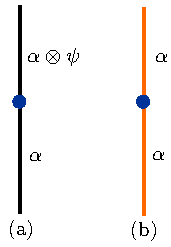
\includegraphics{mvsqtype.pdf}
\caption{ \label{mvsqtype} (a) An m-type particle $\alpha$. The fermion $\psi$ (blue dot) is 
an odd map from $\alpha$ to $\alpha\tp \psi$, with $\alpha\not\cong\alpha\tp\psi$. (b) A q-
type particle $\alpha$ with $\alpha\cong\alpha\tp\psi$, where $\psi$ now acts as an odd 
endomorphism.
%\dave{Should probably use a different letter from $\alpha$ since earlier we use it to denote an `algebra object'?}
%\kw{Seems easier to rename the alg object, which I have done}
%\dave{Sounds good. I thought we used $\alpha$ in section \ref{general_condensation} as an algebra object,
%but that's not the case.}
}
\end{center}
\end{figure} 

It follows from our assumptions about $\psi$ that if $\alpha$ is a simple object of $\mcc$, then
$\alpha\ot\psi$ is also a simple object of $\mcc$.
There are two cases:
\begin{itemize}
	\item If $\alpha\ot\psi$ is not isomorphic to $\alpha$, then $\alpha$ and $\alpha\ot\psi$ are both m-type
	objects of $\mcc/\psi$.
	While $\alpha$ and $\alpha\ot\psi$ represent distinct equivalence classes of simple objects in $\mcc$,
	they belong to the same equivalence class in $\mcc/
	\psi$.
	More specifically, $\alpha$ and $\alpha\ot\psi$ are oddly isomorphic in $\mcc/\psi$, 
	via a digram with a single $\psi$ dot (see Figure \ref{mvsqtype} (a)).
	\item If $\alpha\ot\psi \cong \alpha$, then $\alpha$ becomes a q-type simple object in $\mcc/\psi$.
	The odd endomorphism from $\alpha$ to itself is as shown in Figure \ref{mvsqtype} (b).
\end{itemize}

We will sometimes use the notation
\be
	\sob(\mcc/\psi) = \sobm(\mcc/\psi) \du \sobq(\mcc/\psi) ,
\ee
with $\sobm(\mcc/\psi)$ a complete set of representatives for m-type simple objects, and
$\sobq(\mcc/\psi)$ a complete set of representatives for q-type simple objects.
%\kw{We should drop the above paragraph if we end up not using the notation.}

\medskip

$\mcc/\psi$ is not a braided category, since the back wall used in the condensation procedure 
prevents us from braiding particles completely around one another. 
However, it does have the structure of a front-braiding by $\mcc$, since we are allowed to 
pass $\psi$ worldlines between other particle worldlines and the back wall. 
(Another way of saying this is that $\mcc/\psi$ is a (fermionic) module 2-category for the 3-category $\mcc$.
Yet another way of putting it is that $\mcc/\psi$ is a codimension-1 defect between $\mcc$ and the vacuum.)

\medskip


A particularly simple class of condensed theories obtained from condensing a non-
transparent fermion in a braided theory are provided by the $C_{2(n+1)} = A_{4n+3} / \psi$ series, 
where $A_k$ is the category whose principal graph is the Dynkin diagram of the Lie algebra $\mathfrak{sl}_{k+1}$, 
and $C_k$ is the category whose principal graph is the Dynkin 
diagram of the Lie algebra $\mathfrak{sp}_{2k}$.
The choice $n=0$ 
corresponds to the Ising example considered in Section \ref{C2_condense_sect}. 


%%%%%%%%%%%%%%%%%%%%%%%%%%%%%%%%%%%%%
\subsubsection{Condensing transparent fermions in a braided category}
\label{condense_transparent_fermion}
%%%%%%%%%%%%%%%%%%%%%%%%%%%%%%%%%%%%%

In this subsection we make the same assumptions about $\psi$ and $\mcc$ as in \ref{gntf_condense}, 
but we replace the assumption of non-transparency of $\psi$ with the 
assumption that $\psi$ is transparent in $\mcc$, meaning that it braids trivially with every other particle in $\mcc$.

Since $\psi$ is transparent, we do not need the back wall when performing the condensation.
We still need a spin structure, however (since $\theta_\psi = -1$), and we also need to keep track of 
Koszul signs (since $\psi$ has fermionic statistics).

The resulting category $\mcc/\psi$ is a fermionic braided pivotal category.
The absence of the back wall is what allows for $\mcc / \psi$ to possess a full braiding (rather than the 
``front-braiding'' forced on condensed theories where back walls are needed). 
We will construct an example of such a theory in Section \ref{so36}, where we condense a transparent fermion 
in the $SO(3)_6$ theory.

We note that q-type particles can never arise in the condensed theory if $\psi$ is transparent.
To see this, we note that if $\alpha\ot\psi = \beta$ for $\alpha$ and $\beta$ simple objects of $\mcc$, it follows that 
\be\theta_\beta = \theta_\alpha \theta_\psi = -\theta_\alpha,
\label{noq-type}\ee
where the first equality is because $\psi$ is transparent.
It follows that $\alpha \not\cong \beta$ in $\mcc$, and hence $\alpha$ descends to an m-type 
simple object in $\mcc/\psi$, since if $\alpha$ were q-type we would have $\alpha \tp \psi \cong \alpha$.



%%%%%%%%%%%%%%%%%%%%%%%%%%%%%%%%%%%%%
\subsubsection{Condensing objects that lift to fermions in the Drinfeld Center}
\label{lift_and_condense}
%%%%%%%%%%%%%%%%%%%%%%%%%%%%%%%%%%%%%

%\kw{recent edits in this subsubsection; needs review}

In this section we drop the assumption that $\mcc$ has a braiding.
We will describe how to condense an object $y$ of $\mcc$ which lifts to a fermion in the Drinfeld center $\mcz(\mcc)$. 
%In this section we reduce our assumptions about the object we aim to condense (which we will now refer to as $y$) further. 
%We will not assume that $y\in\mcc$ (for $\mcc$ a UFC) is a fermion, only that it lifts to a fermion in the Drinfeld center 
%$\mcz(\mcc)$. 
An instance of this construction is the $\halfesix$ theory we study in detail in Section \ref{halfesix}.

\medskip

The basic idea is as follows.
The tensor category $\mcc$ can be thought of as a module for the braided category $\mcz(\mcc)$.
In terms of string net pictures, this means that $\mcc$ string nets can be thought of as living on the 2d boundary of a 3d bulk
of $\mcz(\mcc)$ string nets.
We can, if we like, restrict the bulk to only contain strings from a subcategory of $\mcz(\mcc)$, in particular the subcategory
generated by $\unit$ and the lift of $y$.
We can now do the back wall construction on the opposite side of the bulk and proceed as before.
See Figure \ref{ZCPsiCondensed_fig}.
% \nn{need figure}.
\begin{figure}
\begin{centering}
\begin{align}
\begin{array}{ccc}
%\text{(a)} &\quad \quad \quad \quad & \text{(b)} \\[2pt]
\ZCPsiParent &&\ZCPsiCondensed  
\end{array}
\end{align}
\end{centering} 
\caption{\label{ZCPsiCondensed_fig}
%\kw{If we were to rotate the boxes 90 degrees, it might be clearer which strands are on the boundary and which are in the bulk.
%Better color contrast might also help (and would be easier than redrawing a rotated figure).}
%\dave{Oh yea, that color combination is awful. 
%When you say rotated, do you mean have the nets living on top of the box?}
%\kw{I meant rotate 90 deg CW about a vertical axis.  But I think changing the color of the bulk strands should suffice.
%In general, nice fig.}
%\dave{Ok, I'll change the color, and we can discuss on Skype sometime which perspective is our favourite. 
%}
%\dave{How's the contrast now?}
%\ethan{Dave, you continue to outdo yourself with the figures. So amazing!}
%\dave{need to fix braiding between $\psi$s in left box}
On the left we have a 3d box. 
The front of the box is a 2d boundary on which $\mcc$ string nets are drawn (viewed as a module for $\mcz(\mcc)$). 
The bulk of the box contains braided nets from $\mcz(\mcc)$, which we restrict to $\psi$.
The back of the box can be viewed as a trivial boundary to the vacuum.
The right picture shows the box after performing back wall condensation on $\psi \in \mcz(\mcc)$.
The $\psi$ lines terminate on the back boundary at marked points $1,2,3,4$. 
}
\end{figure} 

\medskip

Now for a few more details.

To condense $y$, we first need to lift $y$ to $\mcz(\mcc)$, which means defining half-braidings for $y$. 
For a formal definition of half braid see 
%\cite{muger2003a} and 
\cite{muger2003b} (Definition 3.1 and Lemma 3.3).
A half-braid on an object $y \in \mcc $ is an isomorphism from $y \tp r \rightarrow r \tp y$ for each $r \in \mcc$,
the isomorphism being the half-braiding of $y$ with $r$. 
We will denote these isomorphisms as $e_y(r)$, and write them diagrammatically as
\begin{align} 
e_y(r)  = \halfbraid{\ebox}{y}{r}{}{}.
\label{halfbraid}
\end{align}
One should think of the box braiding $y$ under $r$. 
We could equally well think of this as braiding $y$ over $r$, but since we will use the ``back wall condensation" procedure to condense $y$, 
it is natural to choose $y$ braiding under $r$. 

Using the semisimplicity of $\mcc$ we can write $e_y(r)$ as
\begin{align}
e_y(r)  = \halfbraid{\ebox}{y}{r}{} = \sum_{w \in V^{ry}_{yr}} \left[ e_y(r)  \right]_{w} \halfbraid{\egeneral}{y}{r}{w},
\label{halfbraid_resolution}
\end{align}

Not any isomorphism $e_y(r)$ is allowed; $e_y(r)$ must satisfy some consistency conditions.
For example, braiding with the identity object should be trivial (up to unitors):
\begin{align}
\halfbraid{\ebox}{y}{\mathds{1}}{} = \text{id}_y.
\label{identityBraid}
\end{align} 
The most important property of the braiding isomorphisms is that they commute with fusion, meaning that they can freely slide past the fusion spaces $V^{ab}_c$:
\begin{align}
\halfbraidHex{\HalfBraidHexa}{y}{a}{b}{c} = \halfbraidHex{\HalfBraidHexb}{y}{a}{b}{c}.
\label{junctionBraid}
\end{align}
Taking \eqref{halfbraid_resolution} and inserting it into \ref{identityBraid} and \ref{junctionBraid} allows one to find the $\left[ e_y(r)  \right]_{w}$ defined in \eqref{halfbraid_resolution}. 

In order to do fermion condensation we require $y$ to lift to a fermionic object.
Fermionicity under exchanges means that
\begin{align}
e_y(y) =  -\; \text{id}_y \tp \text{id}_y.
\end{align}
If the quantum dimension of $y$ is 1, then the spin-statistics theorem will imply that the lift of $y$
is also fermionic with respect to twists.

Once a fermion has been defined one can proceed with the techniques of Sections \ref{gntf_condense} and \ref{condense_transparent_fermion}. 
We will provide an example of such a condensation in Section \ref{halfesix}.


%%%%%%%%%%%%%%%%%%%%%%%%
\subsubsection{Condensing non-transparent fermions using spin defects instead of a back wall} \label{spin_defects_condensation}
%%%%%%%%%%%%%%%%%%%%%%%%

In this section, we briefly comment on another way to condense non-transparent fermions through a type of flux attachement, 
which doesn't make use of the back wall construction and allows the condensed theory to remain braided 
(for a braided input category). 
For related ideas, see \cite{kapustin2017,thorngren2015}. 

The construction proceeds schematically as follows.
We allow the $\psi$ worldlines to be absorbed into the vacuum at any point.
In this picture the $\psi$ lines end anywhere in 3-space, they are not restricted to terminating on a back wall. 
In order to resolve problems with the twist and self-statistics of $\psi$, 
we must couple the $\psi$ endpoints to a spin structure and introduce Koszul signs, as before.
This yields an inconsistent theory if $\psi$ is not transparent (see \eqref{transparency_inconsistency}).

However, this inconsistency is rather mild. 
A natural way to distinguish the simple objects in $\mcc$ to use the $\mathbb{Z}_2$ 
grading inherited from the full braid of objects with $\psi$. 
This can be defined by the indicator 
\begin{align} 
(-1)^{\nu_x} := S_{a \psi}/S_{a0} \in \{+1, -1 \}
\label{grading}
\end{align}
It is easy to check that this grading is preserved under fusion.
Hence we can partition the simple objects in $\mcc$ as 
\begin{align} \label{braiding_indicator}
\text{sobj}\; \mathcal{C}  = I_0 \cup I_1,
\end{align}
%where $I_0$ ($I_1$) is the set of simple objects $x$ with $(-1)^{\nu_x} = 1$ ($(-1)^{\nu_x} = -1$).
where $I_k$ is the set of simple objects $x$ with $\nu_x = k$.
%This gives a $\zt$ grading of the simple objects in the theory, and so we have $I_a \tp I_b = I_{a+b\; \text{mod} \; 2}$. 
Since $I_a \tp I_b = I_{a+b\; \text{mod} \; 2}$, this is a $\zt$ grading of the simple objects. 
It can be shown that in any UBFC, $\nu_x = 1$ for all q-type objects (those for which $x\tp \psi \cong x$).
Indeed, if $x$ braided trivially with $\psi$ and $x\tp \psi \cong x$, then it would follow that
$\theta_x = \theta_x \theta_\psi = -\theta_x$, a contradiction.
Therefore, for a given object $a\in\mcc$, $\psi$ must either be transparent with respect to $a$, or be non-transparent only by a minus sign. 

We now observe that the problem in \eqref{transparency_inconsistency} would be 
surmounted if the ``box'' (the physical fermion attached to the $\psi$ endpoint) had a $-1$ 
braiding phase when taken around any anyon with which $\psi$ braids nontrivially. 
This extra $-1$ braiding phase cannot be due to the presence of any additional anyonic 
degrees of freedom, since the physical fermions braid trivially with any emergent anyon. 
However, there's actually a very natural way to do this: bind spin structure defects to the 
worldlines of anyons $x$ with which $\nu_x=1$. 
If the $x$ worldlines get bound to spin structure defects during the condensation 
process, then a box will pick up a factor of $-1$ when traveling around a $x$ line 
(when it passes through the branch cut), which cancels the $-1$ sign from the braiding of 
$x$ and $\psi$, and solves the transparency inconsistency. 
The spin structure defects have $\zt$ fusion rules, and so this procedure is consistent since 
the $\zt$ grading of objects in \eqref{braiding_indicator} is preserved under fusion. 
This allows the condensation to go through without the use of the back wall construction, 
which allows us to perform fermion condensation without sacrificing the existence of a 
braided structure. 

%\kw{Are both D and E comfortable with the claims in this paragraph?}
%\dave{I�m moderately comfortable. 
%I could never figure out how to check it.
%But I don�t see why it would be incorrect.
%}
%\ethan{Yeah, I'm okay with it. I inserted some instances of ``schematically'' in this subsection to make it clear that we aren't pretending to be precise}
This picture also gives us a schematic physical interpretation of how to invert the condensation 
procedure. 
To go the other way and un-condense $\psi$, we just decouple the $x$ lines from the spin structure defects.
This gives us a phase consisting of the MTC $\mcc$ together with a loop gas of spin structure defects.
The loop gas of spin structure defects confine free $\psi$ endpoints, forcing all $\psi$ 
worldlines to be closed and restoring the original phase. 

%\kw{Note to self: add a more mathematical viewpoint to this section.}


%%%%%%%%%%%%%%%%%%%%%%%%%%%%%%%%%%%
\subsection{The tube category of $\mcc/\psi$}
%%%%%%%%%%%%%%%%%%%%%%%%%%%%%%%%%%%

%\ethan{compress a bit---don't hold the reader's hand so much. Can be more concise. }
%\ethan{talk about diffeomorphisms of spin circles and beaurau of standards between spin circles when introducing tube stuff. Maybe write $\tube(X)$ where $X$ is a particular spin circle. Convinient to pick a standard bounding and non-bounding circle. 
%Talk about B and N tube categories and then combine them because we have a tensor product structure.}
%\dave{Note to self: check that we have a definition of minimal idempotent somewhere.
%Refer to it in Section 5.}

The quasiparticle excitations in a bosonic topological phase obtained from a category $\mcc$ 
are given by the simple objects in the Drinfeld center $\mcz(\mcc)$ \cite{levin2005}.
These excitations are also naturally described by primitive idempotents of a category called the tube category of $\mcc$ (see e.g. \cite{ocneanu2001,evans1995,Izumi2000,muger2003b,Bultinck2017,Lan2014, Hu2015}, 
also variously referred to as the tube algebra and the Q-algebra), 
which we will write as $\tube(\mcc)$.

The tube category was first introduced by Ocneanu \cite{ocneanu1994} and has since 
been dubbed ``Ocneanu's tube algebra"; it is also referred to as the annular category $\text{Ann}(\mcc)$, 
or the categorified degree zero Hochschild homology of $\mcc$.
It is closely related to the Drinfeld center:
If $\mcc$ is pivotal then there is a natural isomorphism
$\text{Rep}(\text{Ann}(\mcc)) \cong \mcz(\text{Rep}(\mcc))$, and if $\mcc$ is semisimple then we can drop
the $\text{Rep}$s and obtain $\text{Ann}(\mcc) \cong \mcz(\mcc)$.
With appropriate modifications accounting for spin structure issues, a similar construction holds 
in the more general fermionic setting considered here. 


\medskip

%%KW: this paragraph doesn't really seem necessary to me
%We will now overview the basic idea behind the tube category. 
%Formally, the string-net spin-TQFT construction we have been working with lets us assign a Hilbert space $\mch$
%to an arbitrary spin surface $X$ (the space-time manifold on which our theory lives) with specified string-net boundary conditions. 
%Two surfaces $X$ and $Y$ can be glued together along their boundary components, provided that 
%the boundary conditions and choices of spin structure on these boundary components agree with one another. 
%The manifolds we will consider will always have boundaries that are disjoint unions of circles, and so to 
%study how different manifolds can be glued together, it suffices to specialize to the choice $X = A$, 
%where $A$ is a spin annulus with $\p A = S^1 \du S^1$. 

%The tube category $\tube(\mcc)$ for a string-net TQFT derived from the category $\mcc$ is defined as follows. 
We will now define two categories $\tube^B(\spc)$ and $\tube^N(\spc)$ for a string-net TQFT derived from a given super pivotal category $\spc$. 
We will postpone the most general definition of a super pivotal category until Section \ref{def_sect}. 
However, categories
obtained from fermion condensation $\spc \cong \mcc / \psi$ all constitute examples of super pivotal categories (and provide all the examples of super pivotal categories discussed explicitly in this paper), 
and so the reader may substitute $\mcc/\psi$ for $\spc$ in what follows before reading the more 
general definitions in Section \ref{def_sect}. 

The objects of the two spin tube categories $\tube^B(\spc)$ and $\tube^N(\spc)$ are defined as isomorphism classes of 
string-net boundary conditions on spin circles with bounding 
and non-bounding spin structures, respectively. 
%%KW this remark seems out of place here.  I'm open to moving it elsewhere, but I'm  not sure where.
%Later (see the end of Section \ref{ground_states_on_torus}), we will show that every simple object 
%in $\tube^B(\spc)$ must be m-type. 
For each spin tube category, we will fix a representative spin circle with which to define its
objects. 
Other possible choices of spin circles are related to the chosen representative
by spin diffeomorphisms, and the exact specification of the particular representative will 
be unimportant in our analysis. 
%Because specifying the boundary conditions on a spin annulus involve specifying a choice of spin structure, 
%each object in $\tube(\spc)$ carries a $\zt$ spin structure label according to whether it is associated with the bounding or 
%non-bounding spin structure. 
%This means are two types of objects in the tube category: objects with bounding spin structure
%and ``vortices'', which are objects with non-bounding spin structure.
%Both tube categories may contain both m-type and q-type objects, with q-type 
%objects distinguished by their non-trivial endomorphism algebras as before. 

%The converse is not true, however---in what follows we will see examples of theories with m-type vortices. 

%\kw{Some rewriting starting near here.  D and E might want to review.}
%\dave{re-writes look good. 
%Made some comments on the 2nd-to-last paragraph, should probably discuss with Ethan. 
%}

The morphism spaces of the tube category are finite linear combinations of
spin annuli decorated with different string-net configurations. 
%Spin annuli decorated with different string-net configurations constitute the morphisms of
%the two spin tube categories. 
Again, we will fix a particular representative spin annulus for each spin structure to use
when defining morphisms, with other choices being related by spin diffeomorphisms. 
Figure \ref{ExampleMorphismsTubeC}
%\kw{; includes annuli with multiple endpoints and non-matching numbers of endpoints}
%\dave{Added a figure.} 
shows some examples
of morphisms in the tube category.
\begin{figure}
\begin{centering} 
\begin{align}
\nonumber
\TubeFiga \quad \quad \quad
\TubeFigb  \quad \quad \quad
\TubeFigc  \quad \quad \quad
\end{align}
\caption{\label{ExampleMorphismsTubeC}
Some examples of morphisms in $\tube(\spc)$,
with $\spc$ a super pivotal category obtained through a fermionic quotient ($\spc/\psi$) or more 
generally a category satisfying the assumptions laid out in Section \ref{def_sect}.
We have written the annulus as a square with (unmarked) left and right sides identified. 
At the bottom left of each annulus we have denoted the spin structure of the annulus by B (or N) for bounding (or non-bounding). 
The labels $a,b,c,d \in \sob(\spc)$, and $\nu \in \mor_{\spc}(d \tp b \ra c)$, and $\mu \in \mor_{\spc}(a \ra b \tp d)$.
}
\end{centering} 
\end{figure} 

Up to isomorphism, every object in the tube category is isomorphic to a direct sum of objects with a exactly one string net endpoint on the circle.
Put another way, the full subcategory spanned by such one-endpoint objects is Morita equivalent to the entire category.
This means that for purposes of, for example, enumerating equivalence classes of minimal idempotents or computing Hilbert spaces (ground states),
we can restrict our attention to the one-endpoint subcategory.
And indeed we will usually do so without comment.
(Note however that it is sometimes convenient to work in the larger category; see e.g.\ \ref{mtc_idem_subsect}.)

In the one-endpoint subcategory, morphism spaces can be presented as
\begin{align}
{\rm mor}(\tube^X(\spc))\; =\; \mathbb{C} \left[\AnnularTubexp{\AnnularTubeNoIndex}{a}{b}{c}{d}{\mu}{\nu}{X}{} \right] 
\end{align}
where $a,b,c,d$ are simple objects in $\spc$ and $X\in\{B,N\}$ denotes the spin structure of the annulus. 
The multiplicity indices $\mu$, and $\nu$ are 
collective indices that denote the vector in the fusion space $V^{db}_a$ and $V^{c \bar{d}}_b$, 
as well as the ordering of the tensor product ($V^{d b}_a \tp V^{c d^*}_b$ or $V^{c d^*}_b\tp V^{d b}_a$) which forms the Hilbert 
space of the tube.% (keeping track of this ordering is important because of the Koszul signs incurred 
%when interchanging two odd vectors in a tensor product). 

We define the {\it full} tube category $\tube(\spc)$ to be the direct sum
\be \label{tube_spin_decomp} \tube(\spc) \cong \tube^B(\spc) \oplus \tube^N(\spc).\ee
In what follows we will mostly think of $\tube(\spc)$ as the fundamental category of interest. 
This is because in what follows we will be led to consider a $\tp$ structure on $\tube(\spc)$, which mixes the two spin components (we defer a discussion of this to 
Section \ref{fusion_rules}). 

Composition of morphisms in $\tube(\spc)$ is defined by stacking tubes together.
%The stacking operation plays the role of multiplication 
%in $\tube(\spc)$ when $\tube(\spc)$ is viewed as an algebra. 
Graphically,
\begin{align}
\AnnularTubex{\AnnularTubeNoIndex}{a}{b}{\eta}{X}{} \cdot
\AnnularTubex{\AnnularTubeNoIndex}{c}{d}{\psi}{Y}{} \;
=\; \delta_{X,Y} \delta_{b,c}\AnnulusTubeTubex{\AnnulusTubeTube}{a}{d}{\psi}{\eta}{X}
\end{align}
%\dave{Think this is $\cdot$ notation?}
The $\delta$ functions ensure that if the string labels of the two tubes don't agree on the 
boundary on which they are being glued (i.e. if $b\neq c$), or if the spin structures of the 
two tubes disagree, the two tubes compose (or multiply) to zero. 

%In addition to composing morphisms, we can define a tensor product $\tp$ on $\tube(\spc)$ 
%(from a physical perspective, $\tp$ implements quasiparticle fusion). 
%The definition of $\tp$ is best phrased in terms of vector spaces on the pair of pants, and we defer a 
%discussion of this construction until . 

%%KW I think we discuss the correspondence between (simple) modules and (minimal) idempotents elsewhere
%To actually determine the objects in $\tube(\spc)$, 
%it is helpful to think about the simple objects in $\tube(\spc)$ in terms of vector spaces which are preserved 
%under the action of the morphisms in $\tube(\spc)$\footnote{That vector spaces on circular punctures 
%reproduce $\mcz(\spc)$ makes sense from a formal perspective, as the category $\mcz(\spc)$ is what a 
%(fully-extended) TQFT assigns to an $S^1$.}. 
%If we view $\tube(\spc)$ as an algebra, then these invariant vector spaces correspond precisely to the 
%simple modules $\{M_a\}$ of $\tube(\spc)$.
%This allows us to equivalently classify 
%%Since every simple module $M_a$ of an algebra algebra can be dually represented by a primitive idempotent 
%%$\Pi_a : \tube(\spc) \ra M_a$ that projects onto the vector space $M_a$, we can classify 
%the
%simple objects in $\tube(\spc)$ by the primitive idempotents (projectors whose images are simple modules) $\Pi_a : \tube(\spc) \ra M_a$ of the tube category.%, each of which project onto a different simple module $M_a$ of $\tube(\spc)$.

\medskip

\kw{We also make this point at the end of Section \ref{ss_plaquette_term}, so I suggest that we can be a bit vague here and refer forward
to Section \ref{ss_plaquette_term} for slightly more detail.
Comments welcome.}
\dave{I like it. I think the symmetry bit is left up to interpretation, but I'm fine with that.
I think we could put the first sentence of the second paragraph as a footnote in the first paragraph if we like after the scale transformations sentence.
}

Before moving on, we briefly remark on the physical interpretation of the tube category. 
In Section \ref{Super_pivotal_Hamiltonian} we will define a Hamiltonian whose ground state wave functions assign amplitudes to string nets in such a way
that equivalent string nets receive equal amplitudes.
(In other words, the ground states are naturally identified with the string net TQFT Hilbert space $Z(Y; c)$,
where $Y$ is a spin surface and $c$ is a boundary condition.)
Let $S$ be a boundary component of $Y$, which we will think of as a puncture.
We can act on the space of string nets of of $Y$ (a.k.a.\ $A(Y; c)$) by gluing morphisms of the tube category 
(which are string-net-decorated spin annuli)
to $Y$ at $S$.
Dually, we get an action of the tube category on the ground state vector spaces $Z(Y; c)$ (for various values of $c$).
If we like, we can think of this action of the tube category as a scale transformation; see \cite{Lan2014}.
We can also think of it as a generalized symmetry of the Hamiltonian.
The collection of ground states $Z(Y; c)$ can be decomposed as a direct sum of irreducible representations of the tube category.
The irreducible representations of the tube category are thus identified with the elementary particles (i.e.\ anyons) of the theory.
Using the usual correspondence between minimal idempotents and irreducible representations, we can also identify
the minimal idempotents of the tube category with anyons.
See the end of Section \ref{ss_plaquette_term} for slightly more detail.

Another way of viewing anyons is as local excitations modulo local operators.
From this perspective, the fermionic Drinfeld center (the tube category's close cousin) is relevant.
In the bosonic case, this is explained in \kw{Dave and Paul's paper}\dave{I appreciate the reference to our work, but I don't think it's relevant in this case. 
We only do classical statististical physics in those papers, and just cite math papers when we need to talk about Drinfeld centers.
(It is true that the techniques and results of that paper do generalize to the fermionic case and will be fun to think about.)}.
The techniques used there generalize to the fermionic case, but we will not pursue that in this paper.




\kwsep

\kw{I propose we drop everything below the triple line}

\davex{
\davex{Obviously work in progress.
Having some writers block, will return to this.
I think Haah has a paper where he shows that commuting projector models are tube categories (he doesn't use those words though) }
Possible re-write:
Before moving on, we briefly remark on some physical interpretations of the tube category. 
Depending on perspective, morphisms of the tube category can either be thought of as the set of accessible local operators, or as as ``scale transformations"\cite{Lan2014}. 
...}


\kw{ Will edit the following}

Before moving on, we briefly remark on the physical interpretation of the tube category. 
The setting for examining a collection of $n$ excitations in a given topological phase is a 
manifold decorated with string-nets that possesses $n$ circular punctures (boundary components), with an excitation localized at each puncture.
The type of excitation at a given puncture determines the boundary conditions of the string-net TQFT at that puncture, 
\kw{not really}
and thus the simple objects in $\tube(\spc)$ are identified with the distinct types of quasiparticle excitations that the theory supports. 
%Thus, enumerating the objects of $\tube(\spc)$ amounts to constructing the quasiparticle excitation spectrum of the theory in question. 
\dave{I will do this. (and make note for KW/EL to read it)
These local operators, which can be thought of as scale transformations...}
\ethan{I had a go at it, and tried to strike a balance where we'd both be okay with it}
A helpful physical picture is to think of the morphisms in the tube category as performing local operators
on quasiparticles (which can be thought of as implementing scale transformations on quasiparticles; see \cite{Lan2014}). 
These local operators consist of gluing in string-net-decorated spin annuli (i.e. acting with morphisms in the tube category) to the 
punctures associated with each quasiparticle. 
%\davex{I think it's more clear to replace scale transformation with local operator.
%(The definition of an anyon is `a local excitation modulo local operators'.)
%}
%\kw{let's discuss further on skype}
Since the quasiparticle excitations must be invariant under these local operators\footnote{In this context, we are defining an anyonic excitation to be a local excitation modulo local operators.\dave{Find ref for this definition}} (since they are 
topological, they must be invariant under scale transformations), 
enumerating the quasiparticle excitations in the theory is equivalent to writing down the simple 
modules (or equivalently, the minimal idempotents) of the tube category. 
%\dave{If we go with the morphisms are local operators point of view we could replace the last few sentences with (also disk to puncture?): 
%A potentially helpful physical picture is to think of the morphisms in the tube category as local %operators. 
%These local operators consist of gluing in string-net-decorated spin annuli (i.e. acting with morphisms in the tube category) to the 
%punctures.
%In this picture, 
%we can enumerate the isomorphism classes of anyons by the minimal idemptents (simple modules) of the tube category.}
%}

Of course, the notion of an excitation is strictly speaking not well-defined until we construct a Hamiltonian for the theory.
We will do this in Section \ref{Super_pivotal_Hamiltonian}, but until then we will continue to abuse the word ``excitation''
to refer to an object of the tube category. 
We emphasize that the tube category is a perfectly well-defined mathematical object within 
the formal setting of string-net spin-TQFTs, and the discussion of the tube category 
which follows can be understood without using terms like ``excitation'' and ``Hamiltonian''. 



%%%%%%%%%%%%%%%%%%%%
\subsubsection{Traces and inner products} \label{traces_and_innerproducts}
%%%%%%%%%%%%%%%%%%%%

%\kw{Some rewrites below; D and E should review.}
%\dave{I'm happy with the re-writes. 
%We've also added some examples since the re-writes.}

Recall that a trace on a super linear category $\scat$
%\dave{Was the $C$ on purpose or should we use $\mcc$ instead?} 
%\kw{I have no strong feelings about the letter we use.
%Maybe $\mct$ instead of $\mcc$ since we have the tube category in mind.}
%\dave{That's a good idea. 
%What about keeping the sentence as is and adding a footnote:
%``Often we take $C = \tube(\mcf)$, 
%with $\mcf$ a super pivotal category."
%We use $\mcf$ for a super pivotal category in the definitions section, 
%but I think we should probably choose a different character for that as well (maybe $\mathcal{Q}$).
%}
%\ethan{I think using $\mcc$ and saying ``we often take $\mcc = \tube(\scat)$ with $\scat$ a super pivotal category'' is best. I made a command which is backslash scat for a generic super pivotal category, so that we can decide on the exact letter. It is currently set to $\mcs$ (for super), but we can change it to $\mcf$ or $\mcq$ as well}
%\kw{We often use $\mcc$ for a tensor category, and the discussion in this section is about plain (non-tensor) categories.
%For this reason, I lean against using $\mcc$.
%Are there any objections to $\mct$?}
%\dave{No objections on my end.
%}
%\ethan{Works for me as well}
is an even linear function from endomorphisms to $\cc$, satisfying
\be  \label{trace_cycle_rel}
%	\tr(fg) = (-1)^{|f||g|} \tr(gf) ,
	\tr(fg) = \tr(gf) ,
\ee
for all $f \in \mor(x\to y)$ and $g\in \mor(y\to x)$.
(Note that $\tr(f) = 0$ if $f$ is odd, since $\tr$ is an even function.
Note also that there is no Koszul sign in \eqref{trace_cycle_rel}.)

All of the categories we consider have a reflection structure\footnote{Usually called a $*$-structure,
but we are already committed to denoting the pivotal structure in tensor categories by $*$.}
(more specifically, a pin+ reflection structure),
%\dave{I guess we use two $*$ structures, one for reflection and one for rotation by $\pi$.
%Should we comment on this?} 
which is an order 2 antilinear antiautomorphism of $\scat$
(i.e.\ $\mor(x\to y)$ is sent to $\mor(y\to x)$, for all objects $x$ and $y$).
We will denote the image of a morphism $f$ under reflection as $\bar f$.
The antiautomorphism property has the usual Koszul sign
\be
	\overline{fg} = (-1)^{|f||g|} \overline{g} \overline{f} .
\ee

A trace is equivalent to a collection of sesquilinear inner products on $\mor(x\to y)$ satisfying
\be
	\langle fg, h \rangle =(-1)^{|g||h|} \langle f, h \bar{g} \rangle \;\;\; {\rm and} \;\;\; \langle fg, h \rangle = (-1)^{|f||h|}\langle g,\bar{f}  h  \rangle 
\ee
%\dave{The calculation I'm doing is: 
%\begin{align}
%\langle fg,h \rangle & = \tr(fg\overline{h}) = \tr(f (-1)^{|g||h|} \overline{(h \overline{g})}) = \langle f, h \overline{g} \rangle (-1)^{|g||h|}\\
%\langle fg,h \rangle  &= \tr(fg\overline{h}) = \tr(g\overline{h}f) = \tr(g (-1)^{|f||h|} \overline{(\overline{f}h)}) = \langle g,  \overline{f}h \rangle(-1)^{|f||h|}
%\end{align}
%}
The trace and inner products are related by
\be
\label{trace_to_innerproduct}
	\tr(f) = \langle f, \id_x \rangle   \;\;\; {\rm and} \;\;\;   \langle g,h \rangle = \tr(g\bar{h})
\ee
for $f\in\mor(x\to x)$ and  $g,h\in\mor(x\to y)$.
A trace is called nondegenerate if the corresponding inner product is nondegenerate in the usual sense (on each morphism space individually).

\medskip

We now recall two facts about TQFTs.
The first is that we can define a nondegenerate pairing on the predual Hilbert
space $A(Y; a_1,\ldots,a_k)$, where $Y$ is a spin surface with $k$ disjoint boundary components 
and the $a_i$ are tube category idempotents, satisfying
$\bar a_i = a^*_i$, which specify boundary conditions at each boundary component
%\dave{Can you explain to me what a relection-invariant label is next time we Skype.
%E.g., how come $a_i$ isn't taken to $\bar{a}_i$.}
%\dave{Thanks!}
.
The nondegenerate pairing is defined via
\be
	\langle u, v\rangle = Z(Y\times I) (u\cup \bar v) ,
\ee
where the bar denotes the reflection map from 
$A(Y; a_1,\ldots,a_k)$ to $A(-Y; a_1,\ldots,a_k)$.
%$A(Y; a_1,\ldots,a_k)$ to $A(-Y; \bar{a}_1,\ldots,\bar{a}_k)$
%\dave{bars on $a_i$'s in $A(-Y,....)$?}.
Here we are using the ``pinched boundary" condition for $Y\times I$, so that $\bd (Y\times I) = Y\cup -Y$.
In other words, we glue together the string nets $u$ and $\bar v$ to get a string net on $\bd (Y\times I)$, and then we evaluate
the path integral of $Y\times I$ with the $u\cup \bar v$ string net as the boundary condition.

The second fact concerns the path integral of 3-manifolds of the form $Y\times S^1_B$ or $Y\times S^1_N$.
Let $c$ be a string net on $(\bd Y)\times S^1$ (with either spin structure on $S^1$).
$(\bd Y)\times S^1$ is a disjoint union of tori, and we can cut these tori open into a disjoint union of annuli.
Let $c'$ denote the cut-open string nets on the annuli.
Note that $c'$ is not uniquely determined by $c$; $c'$ depends on where we cut the tori.
The string net $c'$ determines a linear map
\be
	g(c') : A(Y; a_i) \to A(Y; a_i) ,
\ee
given by gluing the $c'$ annuli on to the boundary of a string net on $Y$.
The gluing rules for the path integral imply that
\be
\label{bounding_trace}
	Z(Y\times S^1_B)(c) = \tr(g(c'))
\ee
and
\be
\label{nonbounding_trace}
	Z(Y\times S^1_N)(c) = \str(g(c')),
\ee
where $\str$ denotes the supertrace, which is the trace weighted by the fermion parity operator, i.e. $\str(f) = \tr((-1)^F f)$.
The association of the trace (supertrace) with the $B$ ($N$) spin structure was 
also noticed in \cite{turzillo2016}. 
Note that the partition functions above are independent of the details of the cutting procedure;
any choice of cutting curves and any choice of $c'$ will yield the same answer on the RHS above.

%\kw{Need to make sure we have defined super trace $\str$.}
%\ethan{mentioned it above, should we elaborate more?}
%\dave{We could also just define it in the appendix on 'basic facts about super algebras'.}
%\dave{I think its clear.}

\medskip
We now apply the above to the case where $Y$ is an annulus to obtain a nondegenerate trace on the tube category.
In what follows we will continue to let $\spc$ be a super pivotal fusion category 
satisfying the assumptions of Section \ref{def_sect}
(e.g.~one coming from a fermionic quotient).
Letting $t \in \tube^W(\spc)$ and writing $\tr(t)$ for the trace of $t$, we can use \eqref{trace_to_innerproduct} to write
%\dave{I was thinking we could save $\tr_W(....)$ for traces of matrices i.e., $\tr$ and $\str$ of a matrix for $W = B$ or $W= N$. 
%Then reserve plain old $\tr$ for \eqref{trace_to_innerproduct}. 
%So that the LHS of \eqref{trace_formula} is just $\tr(t)$.}
%\dave{Ethan, if you agree with the change then feel free to comment out the text, if I mis-interpreted something let me know.
%I added an extra sentence below \eqref{trace_formula} explaining the notation.} 
%\ethan{we're on the same page. Added a little more explanation but didn't change the notation}
\begin{align}
\label{trace_t}
\tr (t)  = \langle t, \text{id} \rangle  = Z((S^1_W \times I) \times I ) (t \cup \overline{\text{id} })  = Z(S^1_W \times D^2) (t \cup \overline{\text{id}})
		= Z(S^1_W \times D^2) (\cl(t)) .
\end{align}
%This is the partition function of a solid torus with boundary condition $t \cup \overline{\text{id}}$.
%Sorta confusing since the solid torus only has one boundary component
Diagrammatically we can write the evaluation of the partition function on the right hand side of \eqref{trace_t} as the trace of a matrix, through 
\begin{align}
\label{trace_formula}
\langle t,\text{id}\rangle = \left \langle\;\Tuberrprime_W,\text{id} \; \right \rangle =
 \tr_W \left \{ \Tuberrprimecut \; : A\left(  \PinchedDisk \scriptstyle{x\;} \right)  \xrightarrow{\quad \quad} A \left(  \PinchedDisk \scriptstyle{x\;} \right) 
 \right \}, 
\end{align}
where we have made use of the graphical representation of the endomorphism $t$ in the first equality. 
The solid cylinder in the third equality provides a linear map from the disk at the origin of the $x$ line to the disk at the end of the $x$ line, with each disk 
possessing a single marked point on its boundary labeled  $x$.
The subscript $W$ denotes that the solid cylinder was found by cutting open a cycle with spin structure $W$. 
From \eqref{bounding_trace} and \eqref{nonbounding_trace}, we see that $\tr_W$ will be a trace if $W$ is bounding, and a super trace if $W$ is non-bounding.
The source and target of this linear map is $\text{mor}(\unit \ra x)$, which we write as
the vector space assigned to a disc with one marked point labeled  $x$:
\begin{align}
A\left( \PinchedDisk  \scriptstyle{x\;} \right)  \cong \text{mor}(\unit \ra x) = \bigoplus_i \moronex,
\end{align}
with $\mu_i$ denoting a complete basis of morphisms for $\mor(\unit \to x)$ 
%\ethan{(of course, if $x$ is 
%simple this vector space is zero unless $x\cong \unit$).}
%\kw{shouldn't we remark that this vectos space is zero unless $x \cong \unit$? (assuming $x$ is simple)}
%\ethan{yes}
%With $\mu_i$ denoting a complete basis of morphisms for $\mor(\unit \to x)$.
We allow for $x \cong a_1 \tp a_2 \tp \cdots \tp a_k$ so that a basis of $\mor(\unit \to x)$ could be relatively large.
Often $x$ will denote a simple object 
%(every net configuration on the annulus is isomorphic to one of this form) %%KW sum of things of this form, but I don't think the remark is necessary here
and so $\mor(\unit \to x)$ will be zero or one dimensional: 
%\dave{I think this is OK now.}
\begin{align}
\label{Disk_Hilb}
A \left( \PinchedDisk \scriptstyle{x} \right)  = 
\begin{cases} 
\cc^{1|0} & \text{if $x$ is evenly isomorphic to $\unit$ } \\
\cc^{0|1} & \text{if $x $ is evenly isomorphic to $ \psi$ } \\ 
0 & \text{otherwise} \\
\end{cases}.
\end{align} 
%\kw{I think we need to say ``evenly isomorphic to $\unit$" or something like that; let's discuss best way to say this}
%\dave{I will fix this.}
%\kw{shouldn't we remark that this vectos space is zero unless $x \cong \unit$? (assuming $x$ is simple)}
%\dave{I added a note. 
%Also, when I wrote this I was allowing for $x \cong a_1 \tp a_2 \tp \cdots$, and hence the $\mor(\unit \to x)$ can be non-trivial.
%Is that legitimate? 
%I added a remark on both points.}
%\dave{I added the remark.}

The linear map induced by the cut on these basis elements is given by
\begin{align} 
\moronex \mapsto \moronexcollar = \sum_{j} g_{ij} \; \moronexj.
\end{align}
The coefficients $g_{ij}$ are found by reducing the middle diagram using local relations.
As usual, the trace is basis independent and any basis of $\text{mor}(\unit \ra x)$ will do.

Let us introduce the notation 
\begin{align} \label{sX_defn}
s(X) =\left\{
                \begin{array}{ll}
                  1 \quad &\text{if } X =B \quad \text{Bounding} \\
                  -1 \quad &\text{if } X = N \quad \text{Non-bounding}
                \end{array}
              \right.
\end{align}
Explicitly, \eqref{trace_formula} is then given by
\begin{align} 
\label{matrix_trace}
%\left \langle\;\Tuberrprime_W,\text{id} \; \right \rangle  =
\tr_W(g) = \sum_{ j } g_{jj} s(W)^{|\mu_j|}.
\end{align} 
If $W$ is bounding then $s(W) = 1$ and \eqref{matrix_trace} is just $\tr(g)$. On the other hand, 
if $W$ is non-bounding then $s(W)  = -1$, and \eqref{matrix_trace} is the super trace $\str(g)$. 
%In particular, if $x$ is a simple object then,
%\begin{align}
%\label{Disk_Hilb}
%A \left( \scriptstyle{x\;} \PinchedDisk \right)  = 
%\begin{cases} 
%\cc^{1|0} & \text{if $x \cong \unit$ } \\
%\cc^{0|1} & \text{if $x \cong \psi$ } \\ 
%0 & \text{otherwise} \\
%\end{cases}
%\end{align}
%If $x$ is not a simple object then the super vector space assigned to the disk is $\text{mor}(\unit \ra x)$.
%As usual the trace is invariant under a change of basis, and so any basis will yield the same answer.

This trace is defined for the tube category of any super pivotal category satisfying the assumptions of Section~\ref{def_sect}.
%If $x$ is not simple
%then it is isomorphic to an ordered direct sum of simple objects (assuming semisimplicity) 
%and \eqref{Disk_Hilb} is modified in the obvious way.
%\ethan{added the following}
The inner product obtained from the trace is even, in the sense that $\langle v,w\rangle = 0$ if $|v|\neq|w|$. 
%Furthermore, for the examples we consider later it will be super positive-definite, 
%\kw{how do we know it's super positive definite in the general case?  this seems like something we would want to verify
%in each of our examples, not something that is automatically true because of our other assumptions}
%namely that for all nonzero $v$, we have $\langle v,v\rangle > 0$ if 
%$|v|=0$ and $\langle v,v\rangle/i > 0$ if $|v|=1$. \ethan{this is the usual convention, which makes choosing $A^4=i$ slightly better than $A^4=-i$}
%\dave{Maybe we should move this to where we talk about reflection structure?}
%\kw{I agree we should say something along these lines.  Probably should be moved above; I'll take care of that later.}
%\ethan{we should either move the above or delete the comment on super positive definiteness, which 
%is admittedly kinda contrived anyway}
%\kw{I lean toward just omitting mention of it, mainly because the definition is contrived}
%\dave{That works for me.}

\medskip

%\kw{Probably should also include a summary (glue, rotate 90 degrees, cut, take linear algebra (super) trace}
%\dave{Sounds good, will do this tomorrow.}
%\dave{Still in progress. Will clean up soon.}
%In summary, there is a natural trace defined on the tube category 
%coming from the associated (2+1)-dimensional TQFT.
%Namely, if $t \in \tube^W(\spc)$ is an endomorphism then $\tr(t) = Z(S^1_W \times S^1_B)(\cl_B(t))$. 
%Cutting open the cycle $S^1_W$ results in a string net diagram on the annulus $S^1_B \times I$.
%Denoting the string net on the annuls by $g \in A( S^1_B \times I) $, the TQFT trace $\tr(t)$ 
%is given by a matrix trace of $g$ viewed as an endomorphism of the disk.
%If $W$ is bounding the trace is the standard matrix trace, while if $W$ is non-bounding we use the super trace.
%the annulus of $g$ if $W$ is (non-bounding) bounding. 

%%KW this is the summary I had in mind
In summary, the trace on the tube category is obtained as follows.
Start with a string net $t$ on the annulus $S^1_W\times I$.
Cut $t$ along an interval to obtain a string net on a square.
Rotate this square $\pi/2$ and then reglue (with bounding spin structure) to obtain a new annular string net $\text{rot}(t)$ on $S^1_B\times I$.
Gluing $\text{rot}(t)$ to the boundary of a disk induces a linear map $r_t$ on disk string nets.
If $W = B$ then $\tr(t) = \tr(r_t)$, where the $\tr$ on the RHS is the usual linear algebra trace.
If $W = N$ then $\tr(t) = \str(r_t)$, where the $\str$ on the RHS is the usual linear algebra super trace.
Note that $\text{rot}(t)$ and $r_t$ depend on the choice of initial cut, but $\tr(r_t)$ and $\str(r_t)$ are independent of this choice.


\medskip

%\kw{We should include some sample trace calculations.}
%\dave{Should we do any other examples?}
%\dave{Do you guys think we should join these with the following subsubsection, 
%or leave it as is?}
%\dave{Joined them into this section.}
We now compute some traces that illustrate the techniques 
described in this section, and which will also be of use to us later.

%First, we will compute the total dimension of the category $\scat$.
First we compute the norm squared of a single strand on an annulus with empty boundary conditions.
We denote by $\cl_B(x)$ the closure of $x \in \sob(\spc)$ on an annulus with bounding spin structure:
\begin{align}
\cl_B(x) \; = \; \underset{B}{\clx}
\end{align}
The the norm squared of $\cl_B(x)$ is
\begin{align}
\langle \cl_B(x), \cl_B(x) \rangle = \tr_B \{ \id: \; \mor(\unit \to x \tp x^{*}) \ra \mor(\unit \to x \tp x^*)  \} .
\end{align}
Since $\mor(\unit\ra x\tp x^*) \cong \mor(x\ra x) \cong \End(x)$, we get
 \begin{align}
 \label{clxnorm}
 \langle \cl_B(x), \cl_B(x) \rangle = \dim \End(x) = 
\begin{cases} 
1 & \text{if $x$ is m-type} \\
2 & \text{if $x$ is q-type} 
\end{cases}.
\end{align}

%\dave{This paragraph is newly added.}
%\kw{looks OK to me}
%\dave{Great. Removing comments.}
We can also compute the quantum dimensions $d_{e_j}$ of the minimal idempotents in $\tube(\spc)$.
The un-normalized quantum dimension $\tilde d_{e_j}$ is defined by the trace of the idempotent: 
% tracing out the idempotent:
%defined by the trace of the associated idempotent $\Pi_x$: 
\begin{align}
\tilde d_{e_j} = \tr (e_j),
\end{align}
%where $W$ is bounding if $e_j \in \tube^{B}(\mcc/\psi)$ and non-bounding if $e_j \in \tube^N( \mcc/\psi)$.
The normalized quantum dimension $d_{e_j}$ is then given by $\tilde d_{e_j}/\tilde d_{e_0}$, where $e_0$ is the trivial idempotent.
For example, in the $C_2$ theory, we can use this approach to obtain $\tilde d_{m_{\unit / \psi}} = 1/2, \tilde d_{m_\sigma^+} = \tilde d_{q_{\unit/\psi}} = 1/\sqrt{2}, \tilde d_{q_\sigma} = 1$. 
Normalizing so that $d_{m_\unit} = 1$, we obtain the normalized quantum dimensions listed in Table \ref{C2Data}. 

The total squared dimension $\mcd^2$ of the theory is defined to be 
$ \langle S^2_\phi, S^2_\phi \rangle$, the inner product of the empty diagram on the 2-sphere with itself.
We can then compute
\begin{align}
\langle S^2_\phi, S^2_\phi \rangle = Z(S^2 \times I)(\overline{S^2_\phi} \cup {S^2_\phi}) = \sum_{x \in \sob(\spc)} \frac{Z(B^3, \cl(x)) Z(B^3, \overline{\cl(x)}) }{\langle  \cl_B(x), \cl_B(x) \rangle},
\end{align}
where $B^3$ is the 3-ball and $Z(B^3,\cl(x))$ denotes the partition function 
of a 3-ball with a closed $x$ loop on its surface.
To obtain the second equality, we have written $S^2\times I$ 
as a union of two manifolds homeomorphic to $B^3$ glued along a bounding annulus and 
have made use of the gluing axioms of TQFT. 
We can compute $Z(B^3, {\cl(x)}) = Z(B^3, \overline{\cl(x)}) = d_x$ by definition of the quantum dimension, and hence the total squared dimension is given by
\begin{align}
\label{total_qdim_defn}
\mcd^2 = \sum_{x\in \sob(\spc)} \frac{d_x^2}{\dim \End(x)}.
\end{align} 
%An alternative derivation inspired by fermion condensation is given in Section \ref{Quantum_dimensions}.
%Indeed this calculation is responsible for the denominator in \eqref{XXXX}.

A similar derivation recovers \eqref{non-boundingNullVector}, 
where we pointed out that $\cl_N(\beta)$ is zero.
Let us see how this works out in the tube category $\tube(\spc)$.
Let $x \in \sob(\spc)$, it follows that
\begin{align}
\langle \cl_N(x),\cl_N(x) \rangle  = \tr_N\{ \id: \; \mor(\unit \to x \tp x^*) \ra  \mor(\unit \to x \tp x^*)  \}
= \begin{cases} 
1 & \text{if $x$ is m-type} \\
0 & \text{if $x$ is q-type} 
\end{cases}
\end{align} 
The last equality follows from $\mor(\unit \to x \tp x^*)  \cong \End(x)$ 
and that $\tr_N$ is the super trace of $\id: \; \End(x) \to \End(x)$.
More explicitly,
if $x$ is m-type then as a vector space $\End(x) \cong \cc$ and $\str\{ \id: \; \cc \ra \cc \} = 1$. 
On the other hand, if $x$ is q-type then as a vector space $\End(x) \cong \cc^{1|1}$ and
\begin{align} 
\str \{\id: \; \cc^{1|1} \ra \cc^{1|1} \} = \tr \{(-1)^F: \;  \cc^{1|1} \ra \cc^{1|1} \} =  1-1 = 0
\end{align}
%have non-zero odd vectors and the even and odd part contribute with equal weight but opposite sign (due to the super trace) resulting in $1+(-1) = 0$.
Hence q-type idempotent closed up to an annulus with non-bounding spin structure has norm zero. 
%This provides a nice crosscheck of \eqref{non-boundingNullVector}.
Similarly, one can show that $\langle \cl_N(\gamma), \cl_N(\gamma) \rangle = 2$ 
when $x$ is q-type and gamma is an odd endomorphism such that $\gamma^2 = \id$.

%\dave{Lets also do normalization for closed up idempotents onto the torus.}
%\dave{I am guessing there are many ways to do this calculation, if one of those is simpler and sits in the scope of this section, lets go with that. 
%Otherwise we have the following:}
%Recall from Section \ref{...} when we closed up a q-type idempotent onto the torus we needed to normalize by a factor of $1/\sqrt{2}$ in order to get a unitary S-matrix.
%We compute the modular data for several examples in this paper, to get a unitary S-matrix we need to normalize 
%Lastly we show that the torus has norm squared 
%A fact that we make use of quite often is that a q-type idempotent of the tube category closed up into a torus has norm $\sqrt{2}$.
%See \eqref{XXXX} for an instance of this.

%\dave{KW and EL should double check this with skepticism.}
%\kw{Looks mostly OK to me (after some edits)}
%\ethan{Should we mention somewhere besides here that we assume $r(x) = x$?}
We now show that closing up a q-type idempotent of $\tube(\spc)$ onto a torus results in a state with norm $\sqrt{2}$.
Let $x$ be a minimal idempotent of $\tube(\spc)$, 
and $\cl_W(x) \in A(T^2)$ be the string net found by closing $x$ onto a torus with spin structure $W$ 
along the newly closed cycle. 
%For the moment, assume the newly formed torus is bounding.
First consider the case where $W = B$.
The norm squared of $\cl_B(x)$ is
\begin{align}
\langle \cl_B(x), \cl_B(x) \rangle = Z(T^2 \times I)(\overline{\cl_B(x)} \cup \cl_B(x)) = Z((S^1 \times I)\times S^1_B)(\overline{\cl_B(x)} \cup \cl_B(x)).
\end{align}
%\kw{I think we probably want to assume that $\overline x = x$ and hence $\overline{\cl_B(x)} = \cl_B(x)$}
In the third equality we have rewritten the torus in a form where we can readily apply equation \eqref{bounding_trace} or \eqref{nonbounding_trace}.
The role of $Y$ is played by $S^1 \times I$, an annulus with spin structure determined by $x$.
Further, we can assume a boundary condition given by the idempotent $x$ on each boundary component of the annulus.
We will also assume that $\bar x = x$.
The linear map we need to take the matrix (super) trace of is 
just the identity map, so
%found by cutting open the cycle $S^1_B$. 
%The linear map has an action on $A(S^1 \times I)$ which has a complete basis given by $\End(x)$ treated as a vector space.
%The linear map is only non-trivial on $\End(x)$.
%As in \eqref{clxnorm}, 
%the $W$ dependent matrix trace will be $\dim \End(x)$ (if $\cl_B(x)$ is nonzero) and so 
\begin{align}
\langle \cl_B(x), \cl_B(x) \rangle = \dim \End(x)
\end{align}
A similar calculation for the non-bounding torus yields the same answer, 
however the q-type idempotents need to be closed with an odd endomorphism.
We can now justify the mysterious normalization factor introduced 
in \eqref{closing_q_type_C2} when closing up q-type idempotents on the torus.
A complete orthogonal basis for the torus is given by closing up a complete set of representatives of minimal idempotents.
To find a unitary S-matrix we require each of the basis states to have unit norm,
hence we divide closed up q-type idempotents by $\sqrt{2}$.

%\davex{This paragraph is newly added.}
%\kwx{I think we should rewrite to get rid of any tr that is not related to the tr's above}
%\davex{Agreed.}
%\davex{This has been taken care of, when KW and EL look at it feel free to remove comments.}
%\ethanx{I think the tr's are all correct.}
Lastly we point out a useful relation between the total dimension of a pivotal fusion category $\mcc$ and its fermionic quotient $\mcc/\psi$.
Let $\mcc$ be a pivotal fusion category, $\psi \in \mcz(\mcc)$ a fermion with $\psi \tp \psi \cong \unit$,  and $\mcc/\psi$ the fermionic quotient of $\mcc$,
then
\begin{align}
\label{DC_and_DCpsi}
\mcd_\mcc^2 = 2 \mcd^2_{\mcc/\psi}
\end{align}
if in addition we assume that $\mcc$ is a modular tensor category we also have,
\begin{align}
\label{TubeDim_and_dimCCpsi}
\mcd_{\tube(\mcc/\psi)}^2 = \mcd_\mcc^2 \mcd_{\mcc/\psi}^2
\end{align}
To show \eqref{DC_and_DCpsi}, we simply note 
%\be
%\mcd_\mcc^2 = \tr \left(\bigoplus_{x\in \sob(\mcc)} d_x x\right) = \tr \left( \bigoplus_{x \in \sobm(\mcc/\psi)} d_x (\mathds{1} \oplus \psi) \tp x \right ) + \tr \left(\bigoplus_{x  \in \sobq(\mcc/\psi )} {d_x} x \right),\ee
\begin{align}
\mcd^2_\mcc = \sum_{x\in \sob(\mcc)} d_x^2 = \sum_{x \in \sobm(\mcc/\psi)} d_x^2 + d_{x \tp \psi}^2  + \sum_{q \in \sobq(\mcc/\psi)} d_x^2.
\end{align}
%where $Q$ is the set of all q-type objects in $\mcc$ (those that are invariant under fusion with $\psi$), 
%and $M$ is a collection of representatives of the orbits of m-type objects under fusion with $\psi$, so that 
%the collection of all m-type simple objects is $M\cup M\tp \psi$.   
Since $d_{x \tp \psi}  = d_x d_\psi = d_x$ we can write
\begin{align} 
\label{dimCtoDimCpsi}
\mcd_\mcc^2 =2 \sum_{ x \in \sobm(\mcc/\psi)} d_x^2 + \sum_{x \in \sobq(\mcc/\psi)} d_x^2 = 2 \sum_{x \in \sob(\mcc/\psi)} \frac{d_x^2}{\dim \End(x)} = 2 \mcd_{\mcc/\psi}^2
\end{align} 
%\begin{align}
%\label{dimCtoDimCpsi}
%\mcd_\mcc^2 & = \tr \left( \bigoplus_{x \in \sobm(\mcc/\psi)} d_x (\mathds{1} \oplus \psi) \tp x \right ) + 
%\tr  \left(\bigoplus_{x  \in \sobq(\mcc/\psi)}\frac{d_x}{2}(\unit \oplus \psi) x \right) \\ & =\tr(\unit \oplus \psi) 
%\cdot \tr \left( \bigoplus_{x \in \mcc/\psi} \frac{d_x}{\dim\End(x)} x \right) = \mcd^2_{\rm sVec} 
%\mcd_{\mcc/\psi}^2 = 2 \mcd_{\mcc/\psi}^2,
%\end{align}
hence, \eqref{DC_and_DCpsi}. 
%This result can also be motivated by making use of the theory of modular extensions, see for example \cite{lan2016}\dave{Ethan can you explain this to me.}.
%\ethan{its like de-transparentizing fermions by doing modular extensions. Then we can use results  about how dimensions of modular extensions are products of dimensions of the original category and the extending one}
For the $C_2$ theory, this works out as 
$\mcd_{C_2} = \sqrt{2} = \mcd_{\rm Ising} / \sqrt{2}$.
%Let us summarize the trace descibed in this section. 
%The tube category
Using \eqref{DC_and_DCpsi} and specializing to the case where $\mcc$ is a modular tensor category then $\tube(\mcc/\psi) \cong \mcc \times (\mcc/\psi) $ 
(a result that we prove in Section \ref{double_fermionic_quotient}), and we have 
\be \mcd_{\tube(\mcc/\psi)} = \mcd_{\mcc} \mcd_{\mcc/\psi}.\ee
For example, in the $C_2$ theory this is verified by $\mcd_{\tube(C_2)} = \sqrt{8} = \sqrt{2} (\sqrt{2})^2 = \sqrt{2} \mcd^2_{C_2}.$
%\dave{I suspect that the more general version of this formula holds (i.e., not assuming $\mcc$ to be modular).
%But showing that is somewhat low on my priority list (in the scheme of this paper). 
%Would either of you be embarassed if there was a simple way to show it, 
%and we didn't include the calculation here?
%I would be happy to spend time on it, but there are probably other things to focus on in the paper.
%}


%\dave{commented out things here that we may want to clean up/include, but is not crucial.
%i.e., we could relate inner product of parent theory to condensed theory.}
\begin{comment} 
\dave{Note to self: don't delete this, add to scrap notes.}
If the super pivotal category is derived from a pivotal category $\mcc$ by condensing a fermion,
then we can write the matrix trace in a particularly simple form. \eqref{trace_formula} can be written as
\begin{align}
\label{trace_simple_objects}
\left \langle\;\Tuberrprimenolabel_W,\text{id} \; \right \rangle =  \TuberrTraceCe + s(W) \TuberrTraceCo 
\end{align}
Where the diagram on the right is evaluated in the plane (equivalently, on $S^2$). 
Since the diagram appearing on the right has a trivial lift to the parent category $\mcc$, 
the evaluation is the same whether we use $\mcc$ or $\mcc/\psi$.


Equation \eqref{trace_simple_objects} is useful in its own right. 
It provides a relation between the trace of a tube in $\tube(\mcc)$ and $\tube(\mcc/\psi)$.
Let $\mcc$ be a pivotal fusion category and $\mcc/\psi$ the super pivotal category resulting from condensing a fermion as discussed in Section \ref{General_comments_on_fermion_condensation}.
Then we have have two functors
\be
	\varphi_B : \tube(\mcc) \rightarrow \tube^B(\mcc/\psi)
\ee
and
\be
	\varphi_N : \tube(\mcc) \rightarrow \tube^N(\mcc/\psi) .
\ee
which are inclusions of $\tube(\mcc)$ into $\tube(\mcc/\psi)$.

Recall that the endomorphisms of the trivial object in $\tube(\mcc)$ form a commutative algebra
isomorphic to the fusion ring of $\mcc$, 
and that the $\omega$ loops are the minimal idempotents of this algebra.
We define two non-minimal idempotents in this algebra,
\begin{align}  \label{aJloop}
	a_B = \frac{1}{2}(\cl(\unit) + \cl(\psi)), \;\;\;\;   a_N = \frac{1}{2}(\cl(\unit) - \cl(\psi)),
\end{align}
where as before $\cl(x)$ denotes a closed up $x$ strand embedded in a solid torus.
These two idempotents are orthogonal (i.e.\ $a_I\cdot a_J = \delta_{IJ}a_I$), and $a_B + a_N = \id$.

Placing $a_J$ behind a tube diagram yields a functor $\hat{a}_J : \tube(\mcc) \to \tube(\mcc)$
\begin{align}  \label{aJ_projector}
	\hat{a}_J \left( \TubeBasisa \right) = \TubeProject .
\end{align}
We have a decomposition of $\tube(\mcc)$ into two summands, $\hat{a}_B(\tube(\mcc))$ and $\hat{a}_N(\tube(\mcc))$.
%Thus we have a decomposition of $\tube(\mcc)$ into two summands, $\tube(\mcc)\bullet a_B$ and $\tube(\mcc)\bullet a_N$.
%In pictures, tensoring with $a_J$ looks like
%\begin{align}  \label{aJ_projector}
%	\TubeBasisa \bullet a_J = \TubeProject.
%\end{align}
We also have
\be
	\varphi_I(a_J) = \delta_{IJ} \id ,
\ee
which implies that $\varphi_B\circ\hat a_N$ and $\varphi_N\circ\hat a_B$ are both the zero functor.
It follows that for $t \in a_W(\tube(\mcc))$ we have,
\begin{align}
\label{trace_of_image}
\tr_{\mcc}(t) = \frac{1}{2} \tr_{\mcc/\psi ; W} (t) 
\end{align}
where the subscript in the trace denotes with respect to which category and which spin structure. 
%Said another way, 
%a non-zero tube $t \in \tube(\mcc)$ in the image of $a_W$ has a trivial inclusion into $\tube_W(\mcc/\psi)$, and the traces differ by a the factor of $\frac{1}{2}$ given in \eqref{trace_of_image}.
Indeed, one can show that the functors $\varphi_B\circ\hat a_B$ and $\varphi_N\circ\hat a_N$ are both faithful (i.e.\ injective on morphism spaces).
This is useful when computing the minimal idempotents of 
$\tube(\mcc/\psi)$ given the minimal idempotents of $\tube(\mcc)$, 
as we do in proving Theorem \ref{minimal_idempotents_modular_C/psi}.



%On the other hand, we have:
%$\varphi_B\circ\hat a_B$ and $\varphi_N\circ\hat a_N$ are both faithful:
%It follows that the summand $\tube(\mcc)\bullet a_B$ maps to zero when included in $\tube^N(\mcc/\psi)$,
%and the summand $\tube(\mcc)\bullet a_N$ maps to zero when included in $\tube^B(\mcc/\psi)$.
%With a little more work, we can show that $\tube(\mcc)\bullet a_J$ maps faithfully (injectively) into
%$\tube^J(\mcc/\psi)$ under the functor $\varphi_J$.

%\kw{not satisfied with above; will rewrite soon}
\end{comment} 


\begin{comment}
%%%%%%%%%%%%%%%%%%%%%%%%%
\subsubsection{Quantum dimensions}
\label{Quantum_dimensions}
%%%%%%%%%%%%%%%%%%%%%%%%%



%\dave{Should we call $\tr(e_j)$ the normalized quantum dimension of $\tr(e_j)/\tr(e_0)$ the normalized quantum dimension?}
%\ethan{the latter}
As an application of the trace technology developed in the previous section, we can compute the quantum dimensions $d_{e_j}$ of the minimal idempotents in $\tube(\mcc)$.
The un-normalized quantum dimension $\tilde d_{e_j}$ is defined by the trace of the idempotent: 
% tracing out the idempotent:
%defined by the trace of the associated idempotent $\Pi_x$: 
\begin{align}
\tilde d_{e_j} = \tr (e_j),
\end{align}
%where $W$ is bounding if $e_j \in \tube^{B}(\mcc/\psi)$ and non-bounding if $e_j \in \tube^N( \mcc/\psi)$.
The normalized quantum dimension $d_{e_j}$ is then given by $\tilde d_{e_j}/\tilde d_{e_0}$, where $e_0$ is the trivial idempotent.
For example, in the $C_2$ theory, we can use this approach to obtain $\tilde d_{m_{\unit / \psi}} = 1/2, \tilde d_{m_\sigma^+} = \tilde d_{q_{\unit/\psi}} = 1/\sqrt{2}, \tilde d_{q_\sigma} = 1$. 
Normalizing so that $d_{m_\unit} = 1$, we obtain the normalized quantum dimensions listed in Table \ref{C2Data}. 

%\dave{Could add paragraph about q-type particles having norm $2$?}


We will also need to know how to calculate the total quantum dimension of the theory $\mcd_{\mcc/\psi} = \dim(\mcc/\psi)$.
In bosonic theories we have $\mcd_\mcc^2 = \sum_{x\in \mcc} d_x^2$, where the sum runs over all simple objects $x\in\mcc$. 
This formula is generalized in the fermionic setting, because of the nontrivial endomorphism algebras that simple objects can possess.  
The correct formula is
\be \label{total_qdim_defn} 
\mcd_{\mcc/\psi}^2 = \sum_{x\in \mcc/\psi} \frac{d_x^2}{\dim \End(x)}.\ee
This ensures that $\dim(\mcc)$ is related to $\dim(\mcc / \psi)$ by 
\be \label{DC_and_DCpsi} \mcd_{\mcc / \psi} = \frac{\mcd_\mcc}{\mcd_{\rm sVec}} = \frac{1}{\sqrt{2}} \mcd_\mcc,\ee
where we have viewed the category of supervector spaces, sVec, as consisting of two objects 
${\rm sVec} = \{\unit,\psi\}$ with $d_\unit=d_\psi=1$, so that $\mcd_{\rm sVec} = \sqrt{2}$. 
This result was also obtained in \cite{wan2016}. 

To prove \eqref{DC_and_DCpsi}, we write 
\be
\mcd_\mcc^2 = \tr \left(\bigoplus_{x\in \mcc/\psi} d_x x\right) = \tr \left( \bigoplus_{x \in \sobm(\mcc/\psi)} d_x (\mathds{1} \oplus \psi) \tp x \right ) + \tr \left(\bigoplus_{x  \in \sobq(\mcc/\psi )} {d_x} x \right),\ee
%where $Q$ is the set of all q-type objects in $\mcc$ (those that are invariant under fusion with $\psi$), 
%and $M$ is a collection of representatives of the orbits of m-type objects under fusion with $\psi$, so that 
%the collection of all m-type simple objects is $M\cup M\tp \psi$.   
Since $x\tp \psi \cong x$ if $x\in \sobq(\mcc/\psi)$, we can write
\begin{align}
\label{dimCtoDimCpsi}
\mcd_\mcc^2 & = \tr \left( \bigoplus_{x \in \sobm(\mcc/\psi)} d_x (\mathds{1} \oplus \psi) \tp x \right ) + 
\tr  \left(\bigoplus_{x  \in \sobq(\mcc/\psi)}\frac{d_x}{2}(\unit \oplus \psi) x \right) \\ & =\tr(\unit \oplus \psi) 
\cdot \tr \left( \bigoplus_{x \in \mcc/\psi} \frac{d_x}{\dim\End(x)} x \right) = \mcd^2_{\rm sVec} 
\mcd_{\mcc/\psi}^2 = 2 \mcd_{\mcc/\psi}^2,
\end{align}
proving \eqref{DC_and_DCpsi}. 
This result can also be motivated by making use of the theory of modular extensions, see for example \cite{lan2016}. 
For the $C_2$ theory, this works out as 
\be \mcd_{C_2} = \sqrt{2} = \mcd_{\rm Ising} / \sqrt{2},\ee
and is easily checked to hold for the other examples in the $A_{4n+2} / \psi$ series.  

It is a result of Muger \cite{muger2003b} that for any unitary fusion category $\mcc$, 
the dimension of the center is related to $\mcd_\mcc$ by 
\be \mcd_{\tube(\mcc)} =\mcd^2_\mcc.\ee
One can ask for the analogous formula in the super pivotal case.
We can then use \eqref{DC_and_DCpsi} to obtain 
\be \mcd_{\tube(\mcc)} = 2\mcd^2_{\mcc/\psi}.\ee
Using \eqref{DC_and_DCpsi} again and specializing to the case where $\mcc$ is a modular tensor category then $\mcc \times (\mcc/\psi) \cong \tube(\mcc/\psi)$ 
(a result that we prove in Section \ref{double_fermionic_quotient}), we have 
\be \mcd_{\tube(\mcc/\psi)} = \mcd_{\mcc} \mcd_{\mcc/\psi}.\ee
For example, in the $C_2$ theory this is verified by $\mcd_{\tube(C_2)} = \sqrt{8} = \sqrt{2} (\sqrt{2})^2 = \sqrt{2} \mcd^2_{C_2}.$



\medskip

\dave{Below is old stuff (commented out). 
Should decide if we want to keep anything else from it, I think most of it has been copied over.}

\end{comment}

\begin{comment} 
In what follows we will need to compute the trace of a generic operator (or in other words, an endomorphism) $\mco$ in the tube category. 
\kw{I think we should say endomorphism rather than operator, and use lower case notation for this operator.}
We will do the computations following the procedure outlined in \cite{Walker2006}; for more details see \cite{ghosh2016,das2014}.
\dave{I think at one point I thought those two references might be useful, but not so sure anymore.}
\kw{If you think the other two refs are useful and relevant, include them; otherwise not.}

To compute the trace of a endomorphsism in $\mcc$ (which can be thought of
as string nets on a disk), we identify the incoming and outgoing
boundaries of the disk to get a string net on $S^2$.
We then use the standard evaluation for $S^2$ string nets to get a number.
For an endomorphism $\mco$ in $\tube(\mcc)$, we follow the same procedure by identifying the incoming and outgoing
boundaries of the annulus, yielding a string net on the torus.
There is no standard evaluation for string nets on the torus (it is not 1-dimensional vector space in general),
but TQFT considerations pick out a preferred map from torus string nets to $\cc$, as we describe below.


\kw{I will rewrite below}

\kw{Note to self: be sure to introduce inner product (more general than trace)}

\kw{should probably make some observations needed for proof of lemma in MTC/psi section}



\dave{Do the two agree at the level of the tube category?
(i.e., I thought $\langle X, Y \rangle  = \langle \unit ,X^*Y\rangle = \text{tr} X^*Y$.
I used this fact later in \ref{image_aJ} but can also do the same calculation without it.)}

Recall that the path integral on a manifold $X$ is a linear function
\be Z(X) : V(\p X) \ra \cc,\ee
where $V(\p X)$ is the set of all string-net configurations on $\p X$ modulo local relations.
The trace of an operator supported on a manifold $Y$ is equal to the partition function on a manifold $X$ 
such that $\p X = Y$ evaluated on the string-net configuration specified by that operator. 
For our application to the tube category, we thus have 
\be {\rm Tr}\ \mco = Z(S^1 \times D^2)(\mco),\ee
where $S^1\times D^2$ is the solid torus. 

To compute this partition function, we make use of a cutting trick. 
We use the relation 
\be {\rm Tr}_Y\ (Z(X_{cut})) = Z(X_{glue}).\ee
In the above formula, $X_{cut}$ is a manifold which becomes $X_{glue}$ after gluing $X_{cut}$ by pasting in 
$Y$ along the boundary components of $X_{cut}$, and the ${\rm Tr}_Y$ instructs us to sum over all such $Y$.
This is illustrated in Figure \ref{cutting_trick}. The leftmost figure is a solid torus, on which an operator $\mco$ is supported. 
We then cut the torus as shown in the second step, and glue it together again as shown in the last step. 
We see that at the end of these steps, we have rotated the string-net configuration of the operator $\mco$ by $\pi/2$.
Therefore, we find
\begin{align}
\text{Tr} \; \mco &= {\rm Tr}\ (R_{\pi/2}(\mco)),
\end{align}
where $R_{\pi/2}(\mco)$ is the operator $\mco$ after having its string-net configurations have been rotated counterclockwise by $\pi/2$.
Schematically, this can be written as
\begin{align}
\text{Tr}\ \AnnulusGeneric = \text{Tr}\;  \left( \RotatedTube : \Disc \ra \Disc \right)
\end{align}
Despite the abstract nature of this discussion, the calculation of traces is easy in practice: to compute 
the trace of a tube, we rotate the string-net configuration on the tube by $\pi/2$ counterclockwise, 
identify the top and bottom of the tube, and simplify the resulting diagram. The trace is then found by 
taking the coefficient of the final diagram. 
\begin{figure}
\begin{center}
\begin{align}
\xymatrix @!0 @M=1mm @R=7mm @C=30mm {
\AnnulusGeneric \ar[r]^{\text{cut}}& \AnnulusCut \ar[r]^{\text{id}} & \AnnulusFlat \ar[r]^{\text{glue}}& \RotatedTube}
\end{align}
\caption{ \label{cutting_trick} Defining the trace of the tube by taking the inner product with the identity tube.
The first step is to cut open the annulus along the azimuthal cycle. 
then glue the inner and outer intervals together to get a rotated tube, shown at the far right.
We then view this rotated tube as a linear map from $D^2$ to $D^2$, and the trace of this map is the trace of the tube.
}
\end{center}
\end{figure}



Now that we know how to take traces and map string-nets on the torus to $\cc$, we are equipped with a way 
of taking inner products between morphisms in the tube category. To form the inner product $\langle u,v\rangle$, 
we take the annuli corresponding to $u$ and $v$, identify their boundaries together to form a torus, 
and use our tracing procedure to map this string-net torus to a complex number, which we identify with $\langle u,v\rangle$. 

The quantum dimension $d_x$ of an excitation $x$ in $\tube(\mcc)$ is defined by the trace of the associated idempotent $\Pi_x$: 
\begin{align}
d_x \equiv \text{Tr} (\Pi_x).
\end{align}
For example, in the $C_2$ theory, we can use this approach to obtain $d_{m_{\unit / \psi}} = 1/2, d_{m_\sigma^+} = q_{\unit/\psi} = d/2, q_\sigma = 1$. 
Normalizing so that $d_{m_\unit} = 1$, we obtain the quantum dimensions listed in Table \ref{C2Data}. 

We will also need to know how to calculate the total quantum dimension $\mcd_\mcc = \dim(\mcc)$.
In bosonic theories we have $\mcd_\mcc^2 = \sum_{x\in \mcc} d_x^2$, where the sum runs over all simple objects $a\in\mcc$. 
This formula is generalized in the fermionic setting, because of the nontrivial endomorphism algebras that simple objects can possess.  
The correct formula is
\be \label{total_qdim_defn} \mcd_{\mcc/\psi}^2 = \sum_{x\in \mcc/\psi} \frac{d_x^2}{\dim \End(x)}.\ee
This ensures that $\dim(\mcc)$ is related to $\dim(\mcc / \psi)$ by 
\be \label{DC_and_DCpsi} \mcd_{\mcc / \psi} = \frac{\mcd_\mcc}{\mcd_{\rm sVec}} = \frac{1}{\sqrt{2}} \mcd_\mcc,\ee
where we have viewed the category of supervector spaces, sVec, as consisting of two objects 
${\rm sVec} = \{\unit,\psi\}$ with $d_\unit=d_\psi=1$, so that $\mcd_{\rm sVec} = \sqrt{2}$. 
This result was also obtained in \cite{wan2016}. 



To prove \eqref{DC_and_DCpsi}, we write 
\be
\mcd_\mcc^2 = \text{Tr} \left(\bigoplus_{x\in \mcc/\psi} d_x x\right) = \text{Tr} \left( \bigoplus_{x \in M} d_x (\mathds{1} \oplus \psi) \tp x \right ) + \text{Tr} \left(\bigoplus_{x  \in Q} {d_x} x \right),\ee
where $Q$ is the set of all q-type objects in $\mcc$ (those that are invariant under fusion with $\psi$), 
and $M$ is a collection of representatives of the orbits of m-type objects under fusion with $\psi$, so that 
the collection of all m-type simple objects is $M\cup M\tp \psi$.   
Since $x\tp \psi \cong x$ if $x\in Q$, we can write
\begin{align}
\label{dimCtoDimCpsi}
\mcd_\mcc^2 & = \text{Tr} \left( \bigoplus_{x \in M} d_x (\mathds{1} \oplus \psi) \tp x \right ) + 
\text{Tr}  \left(\bigoplus_{x  \in Q}\frac{d_x}{2}(\unit \oplus \psi) x \right) \\ & =\text{Tr}(\unit \oplus \psi) 
\cdot \text{Tr} \left( \bigoplus_{x \in \mcc/\psi} \frac{d_x}{\dim\End(x)} x \right) = \mcd^2_{\rm sVec} 
\mcd_{\mcc/\psi}^2 = 2 \mcd_{\mcc/\psi}^2,
\end{align}
proving \eqref{DC_and_DCpsi}. 
This result can also be motivated by making use of the theory of modular extensions, see for example \cite{lan2016}. 
For the $C_2$ theory, this works out as 
\be \mcd_{C_2} = \sqrt{2} = \mcd_{\rm Ising} / \sqrt{2},\ee
and is easily checked to hold for the other examples in the $A_n / \psi$ series.  

It is a result of Muger \cite{muger2003a,2003b} that for any unitary fusion category $\mcc$, 
the dimension of the center is related to $\mcd_\mcc$ by 
\be \mcd_{\tube(\mcc)} =\mcd^2_\mcc.\ee
We can then use \eqref{DC_and_DCpsi} to obtain 
\be \mcd_{\tube(\mcc)} = 2\mcd^2_{\mcc/\psi}.\ee
Using \eqref{DC_and_DCpsi} again and using $\mcc \times (\mcc/\psi) \cong \tube(\mcc/\psi)$ (a result 
that we prove in Section \ref{double_fermionic_quotient}), we have 
\be \mcd_{\tube(\mcc/\psi)} = \sqrt{2}\mcd^2_{\mcc/\psi}.\ee
For example, in the $C_2$ theory this is verified by $\mcd_{\tube(C_2)} = \sqrt{8} = \sqrt{2} (\sqrt{2})^2 = \sqrt{2} \mcd^2_{C_2}.$





\subsubsection{\dave{May salvage some material from this, but otherwise may be removed.}}


%First, any string net configuration of the parent theory descends to a string net configuration of the condensed theory.

%giving us a functor $\tube(\mcc) \rightarrow \tube(\mcc/\psi)$.
%Conversely, we can always take an even morphism in $\mcc/\psi$ and lift it to $\mcc$, giving 
%us a way from lifting tubes in $\tube(\mcc/\psi)$ to those in $\tube(\mcc)$.
%These two facts allow us to find the minimal idempotents of the quotient theory, 
%using the minimal idempotents of the parent theory.



%\dave{I haven't checked the above, will come back to it.}
%\kw{Looks OK to me.}

%The proof of the theorem splits into two parts. 
%We first compute the images of the minimal idempotents in $\tube(\mcc/\psi)$ under condensation
%and show that these images provide us with a complete set of minimal idempotents in the condensed theory.
%Next we define a tensor functor from $\mcc \times \overline{\mcc/\psi} $ to $\tube(\mcc/\psi)$ and
%show that it is an isomorphism of tensor categories.
%thus showing that $\tube(\mcc/\psi) \cong \mcc \times \overline{\mcc/\psi}$ as tensor categories.
\end{comment} 

\begin{comment} %%%%%%%%%%%%%%%%

The image of the idempotents in $\tube(\mcc)$ under condensation can be found with the help of 
two projectors $a_B,a_N$ which sum to the identity, and are defined to act on morphisms in $\tube(\mcc/\psi)$. 
They are defined as
\begin{align}
a_B = \frac{1}{2}(\cl(\unit) + \cl(\psi)), \;\;\;\;   a_N = \frac{1}{2}(\cl(\unit) - \cl(\psi)),
\label{aJloop}
\end{align}
where as before, $\cl(x)$ denotes a closed up $x$ strand embedded in a solid torus.
Importantly, they satisfy $a_J \tp a_W = \delta_{JW} a_J$ and $a_B + a_N = \cl(\unit)$\footnote{
By ${\rm cl}(a)\tp{\rm cl}(b)$, we mean ${\rm cl}(a\tp b)$.}.
Also, from the definition of the $\omega$ loop we note that $\omega\tp a_J = \delta_{J,B}\omega$. 
Notice that an $a_J$ loop encircling a tube with spin structure $J$ is the identity, while an $a_J$ loop 
on a tube with spin structure $W \neq J$ projects the tube to zero.
That is, 
\begin{align}
\SpinStructureProjector = \delta_{JW}\; \EmptyTubeW \in \tube^W(\mcc/\psi),
\end{align}
where $W$ on the interior of the gray disc denotes the spin structure for the disc it bounds.

The projectors can also be defined to act on morphisms in $\tube(\mcc)$. In this setting we will denote 
them as $\hat{a}_B$ and $\hat{a}_N$. 
On general morphisms in $\tube(\mcc)$, they act as 
\begin{align}
\hat{a}_J \cdot \TubeBasisa = \TubeProject.
\label{aJ_projector}
\end{align}


The $\hat{a}_J$ projectors allow us to determine which idempotents in $\tube(\mcc)$ survive the projection 
to $\tube(\mcc/\psi)$:
a non-zero tube in $\tube(\mcc)$ in the image of $\hat{a}_J$ remains non-zero under condensation as a tube in $\tube^J(\mcc/\psi)$. 
We make this precise in the following lemma:

\end{comment} %%%%%%%%%%%%%%%%


\begin{comment}

\begin{lemma}  \label{image_aJ}
The functors $\varphi_B\circ\hat a_B$ and $\varphi_N\circ\hat a_N$ are both faithful (i.e.\ injective on morphism spaces).
\end{lemma}

%\begin{lemma}
%\label{image_aJ}
%Let $\mcc$ be a modular tensor category and $\psi$ a fermion in $\mcz(\mcc)$ as defined in \ref{lift_and_condense}.
%Let $\hat{a}_J$ be as defined in \eqref{aJ_projector}.
%Then there exists a functor 
%\[\begin{tikzcd}        
%   I: \hat{a}_J \cdot \tube(\mcc) \rightarrow \tube^J(\mcc/\psi)
%\end{tikzcd}\]
%which is faithful, meaning that morphisms in $\hat{a}_J\cdot\tube(\mcc)$ are mapped injectively to morphisms in $\tube^J(\mcc/\psi)$. 
%\ethan{may still need to be rephrased}
%In particular, a tube of $\tube(\mcc)$ that is not mapped to zero by $\hat{a}_J$ is nonzero in the image of $I$. 
%\end{lemma}

\kw{I'm skipping the proof of the lemma; will come back later}

\begin{proof}
The proof follows from a simple observation.
Let $t \in \tube(\mcc)$ be in the image of $\hat{a}_J$ so that, 
\begin{align}
\left \langle\; \Tubeidr,\Tuberr \; \right \rangle_{\tube(\mcc)} &=\left \langle\; \Tubeidr,\TuberraJ \; \right \rangle_{\tube(\mcc)}  \\
&= \frac{1}{2} \left \langle  \TuberrTraceCe + (-1)^{s(J)} \TuberrTraceCo  \right \rangle_{\mcc}
\end{align}
The first step follows from $t$ being in the image of the projector $\hat{a}_J$, 
while the second step follows from the definition of the inner product in the tube category 
(written as $\langle,\rangle_{\tube(\mcc)}$, which is discussed in Section \ref{traces_and_innerproducts}). 
The angle brackets with subscript $\mcc$ in the second line means that we evaluate the picture on 
the two-sphere using local relations in $\mcc$.
As before, we have defined $s(J)= 0$ if $J$ is bounding and $s(J)=1$ otherwise.

Since any net configuration in $\mcc$ evaluated on $S^2$ agrees with the evaluation in $\mcc/\psi$ we have,
\begin{align}
\frac{1}{2} \left \langle  \TuberrTraceCe + (-1)^{s(J)} \TuberrTraceCo  \right \rangle_{\mcc} &=\frac{1}{2} \left \langle  \TuberrTraceCe + (-1)^{s(J)} \TuberrTraceCo  \right \rangle_{\mcc/\psi} \\
&= \frac{1}{2} \left \langle\; \Tubeidr,\Tuberr \; \right \rangle_{\tube^J(\mcc/\psi)},
\end{align}
where we have again used the definition of the trace. 
Hence, if $X,Y \in \tube(\mcc)$ are in the image of $\hat{a}_J$, then $\langle X, Y \rangle = \langle \unit, X^* Y\rangle$. 
Using that $\tube(\mcc)$ is semi-simple, and that the $t \in \tube(\mcc)$ above span all 
morphisms of $\tube(\mcc)$, we can always find an isomorphism such that $t \cong X^*Y$.
\ethan{I'm confused by the last two sentences and why we need them}
\dave{If a tube $X$ is non-zero in $\tube(\mcc)$, then $\langle X, X\rangle$ is non-zero (I'm assuming the 
inner product is non-degenerate for both $\tube(\mcc)$ and $\tube(\mcc/\psi)$. 
Not all tubes in $\tube(\mcc)$ look like $t$ above, so we need to say that they are all isomorphic 
to one that looks like $t$. 
I think that in order for that to be true $\tube(\mcc)$ should be semi-simple, 
but this I'm not certain of.
}
From the previous equation we have that $\langle X, Y \rangle_{\tube(\mcc)} = \frac{1}{2} \langle X, Y \rangle_{\tube^J(\mcc/\psi)}$.
Since the the inner product is non-degenerate \ethan{did we prove this?}
\dave{No, not yet.
I assumed in the next re-write of the inner product section we would either mention it's non-degenerate with a reference, or prove it.
Otherwise we could re-word the above.}, the inclusion of $\hat{a}_J\cdot\tube(\mcc)$ into $\tube^J(\mcc/\psi)$ is injective on morphisms.
\end{proof}



Let's now apply the $\hat a_J$ functors to the idempotents in the parent theory $\tube(\mcc)$. 
%Define the image of $e_{xy}$ under condensation to be $f^J_{xy}$. 
Define
\be
	f^J_{xy} = \varphi_J(e_{xy}) .
\ee
Using that $\omega \cdot a_J = \delta_{JB} \omega$, we can replace the $\omega$ appearing in $e_{xy}$ with $a_B \cdot \omega$. 
We can next pass the $a_B$ through the $y$ strand sitting between the $\omega$ loop and the back wall. 
Doing so permutes $a_B$ and $a_N$ if $y$ has nontrivial braiding with $\psi$.
Otherwise $a_B$ remains unchanged (if $y$ braids trivially with $\psi$). 
Diagrammatically, 
\begin{align}
e_{xy} =  \TubeIdempotentTwoStrand= \exyomegaa = \begin{cases}
\exyomegac& \text{if}\; \nu_y = 0 \\
\\
\exyomegab& \text{if}\; \nu_y =1
\end{cases},
\end{align}
\kw{We can also see the above more directly, since we are free to insert $a_J$ in an annular diagram with spin structure $J$.}
where the indicator $\nu_y$ is defined as before by $\nu_y=0$ if $y$ braids trivially with $\psi$, and $\nu_y=1$ otherwise. 
This means that each $e_{xy}$ has an image in $\tube(\mcc/\psi)$ given by
\begin{align}
e_{xy} \xrightarrow{\text{condense $\psi$}}f_{xy}^{J(y)} \quad \quad \text{with $J(y) = B$ if $\nu_y = 0$ and $J(y) = N$ otherwise}
\label{image_of_exy}
\end{align}
\kw{Is previous statement redundant?}
In the following we will sometimes write just $J$ instead of $J(y)$. 
Since the $e_{xy}$ are complete, orthogonal and non-zero then by using the Lemma \ref{image_aJ}
we also have that the $f^J_{xy}$ are complete, orthogonal and non-zero\footnote{they are complete since all the non-zero even 
tubes in the condensed theory lift to non-zero tubes in the parent theory, meaning that we are not ``missing'' any 
idempotents after projecting the idempotents in the parent theory to the condensed theory.}.
Note that the inclusion of the image of $\hat{a}_J$ in $\tube^J(\mcc/\psi)$ is not surjective: 
indeed, tubes that have $\psi$ lines terminating on the interior of the tube do not appear in $\tube(\mcc)$.
For example a tube with a q-type strand could always have a $\psi$ line extending from it and terminating on the back wall.
Hence, we also need to show that the resulting idempotents are minimal.
\end{comment}

%%%%%%%%%%%%%%%%%
\subsubsection{The sum-of-squares formula}
%%%%%%%%%%%%%%%%%

%\ethan{Okay, the version that follows has been expanded on to include more explicit stuff later on. 
%KW and DA should check}
%\kw{looks OK to me}
%\dave{I'll read through it and delete comments.}
%\dave{Looks good to me. Changed primitive to minimal, and added `and their type' to the last sentence.}

When analyzing tube categories, we are often presented with a collection of non-simple objects $x_1, x_2, \ldots$
(e.g.~single string net endpoints), together with the super dimensions of the vector spaces $\mor(x_i\to x_j)$.
From this we want to deduce a complete set of minimal idempotents $\{e_\alpha\}$, together with isomorphisms
\be \label{xi_decomp}
	x_i \cong \bigoplus_\alpha W_{i\alpha} \cdot e_\alpha 
\ee
where the $\{W_{i\alpha}\}$ are supervector spaces. 
We will show in \eqref{amordef} how to compute morphism spaces between objects that are 
of the form of those in the RHS of \eqref{xi_decomp}. 
Applying \eqref{amordef} yields
\be  \label{coldotprod}
	\mor(x_i\to x_j) \cong \bigoplus_\alpha \Hom(W_{i\alpha} \to W_{j\alpha})\otimes_\cc \End(e_\alpha) .
\ee
When $i\ne j$, this is merely an isomorphism of supervector spaces, but when $i = j$ this is an isomorphism of super algebras.

It is frequently possible, given the left hand side of \eqref{coldotprod} and a small amount of additional information, 
to solve for the things on the right hand side: the idempotents $\{e_\alpha\}$, their types, and the coefficients $W_{i\alpha}$.
This is useful since the morphisms that constitute the left hand side are often very easy to enumerate: they are simply the different tubes in $\tube_{x_i\ra x_j}$. 
In terms of super dimensions, setting $i=j$ we have 
\be \label{sum_of_squares} \dim(\mor(x_i\ra x_i)) = \sum_\alpha \dim(\End(W_{i\alpha}))\dim(\End(e_\alpha)).\ee
This is a fermionic ``sum-of-squares'' formula since $\dim\,\End(W_{i\alpha})$ will always be the square of 
an integer. 

For example, we can consider the space $\mor^X(\unit\ra\unit)$ in the $C_2$ theory.
Letting $X=B$ we see immediately from \eqref{mortube} that $\mor(x_i\ra x_i)$ has super dimension $2|0$, meaning that there must be two summands on the RHS of \eqref{sum_of_squares}, and hence 
two minimal idempotents in $\tube^B_{\unit\ra\unit}$. Letting $X=N$ we read off a super dimension of $1|1$, which implies that there is only one q-type idempotent in $\tube^N_{\unit\ra\unit}$. 
Similarly from \eqref{mortube} one verifies that the super dimensions of $\mor^X(\beta\ra\beta)$ 
are each $2|2$, meaning that each sector must contain either one m-type idempotent with $\dim\End(W_{\alpha})=2^2$ or two q-type idempotents $e_\alpha$ with 
$\dim\End(W_{\alpha})=1$ (although the latter is ruled out if $X=B$ since $\tube^B$ can 
host no q-type idempotents).
Thus, one can learn a good deal about the number of minimal idempotents and their type in the tube category 
simply from a list of the non-zero linearly independent tubes. 

In Section \ref{he6mp-tube-cat} we will see a further example of these techniques.


%%%%%%%%%%%%%%%%
%%%%old sum of squares stuff
\begin{comment}
\kwsep

In this section, we briefly present a fermionic version of the sum-of-squares formula, which is useful for relating the dimension
of the tube category to the dimensions of its minimal idempotents (see e.g. \cite{Lan2014}). 
In many cases, this allows us to obtain a large amount of information about the quasiparticle 
content of the theory without actually finding the explicit representations of the primitive 
idempotents of the tube category.

If $\{e_a\}$ is a list of isomorphism classes of minimal idempotents of $\tube(\mcc/\psi)$, 
%(recall that these are in one-to-one correspondence with quasiparticles, otherwise known as %isomorphism class of minimal idempotents of the tube category), 
then 
the sum-of-squares formula reads
\be \label{sumofsqs} \dim \tube(\mcc/\psi) = \sum_{e_a \text{ m-type}} (\dim e_a)^2 + 2\sum_{e_a \text{ q-type}} (\dim e_a)^2,\ee
where the factor of 2 in front of the second sum comes from the fact that if $a$ is q-type, 
the even and odd parts of the image of $e_a$ have equal dimensions (as they are oddly isomorphic). 
The left hand side of the above formula is simply the number of non-zero linearly independent tubes in $\tube(\mcc/\psi)$, which 
is typically very easy to compute. 
If there are no q-type particles in $\tube$ then there are no terms in the second sum on the right hand side, 
and we reproduce the bosonic sum-of-squares formula.  

As an example, we can consider the $C_2$ theory. 
There are three q-type minimal idempotents (all in the $\tube^N$ sector) and three m-types (all in the $\tube^B$ sector). 
All of the minimal idempotents are one-dimensional with the exception of $m_\sigma$, 
which is the two-dimensional isomorphism class of $m_\sigma^+$ and $m_\sigma^-$. 
Since there are 12 linearly independent tubes in $\tube(C_2)$ (see \eqref{atubes} and \eqref{ptubes}), 
the sum-of-squares formula then reads
\be 12 = 1^2+2^2+1^2+2(1^2+1^2+1^2).\ee
\end{comment}
%%%%%%
%%%%%%


%%%%%%%%%%%%%%%%%%%%%%%%%
\subsection{Ground states on the torus} \label{ground_states_on_torus}
%%%%%%%%%%%%%%%%%%%%%%%%%

In what follows, we will let $T_{XY}$ with $X,Y\in\{B,N\}$ denote the torus with spin structure $XY$
(with spin structure $X$ along the meridional cycle and $Y$ along the longitudinal cycle),
and $A(T_{XY})$ 
%\kw{might want to switch this to $A(T_{XY})$}
the Hilbert space of ground-state string-net configurations on $T_{XY}$.  
As before, we will also let $\tube^B$ denote the bounding tube category and $\tube^N$ denote the non-bounding tube category. 

We have the following theorem, valid for any super pivotal category, which allows us to determine 
the ground states on a torus from the tube category:

\begin{theorem} \label{torus_basis_theorem}
Let $X$ equal $B$ or $N$.
The Hilbert space $A(T_{XB})$ is purely even, with an orthogonal basis given by closed-up idempotents $\{\cl(e_i)\}$,
where $e_i$ runs through a set of representatives of the minimal idempotents of $\tube^X$.
The Hilbert space of $T_{XN}$ is isomorphic to $\cc^{p|q}$, where $p$ is the number of m-type idempotents of $\tube^X$
and $q$ is the number of q-type idempotents of $\tube^X$.
An orthogonal basis is given by $\{\cl(e_i)\}$, where $e_i$ runs through a set of 
representatives of the minimal m-type idempotents of $\tube^X$,
union $\{\cl(\gamma_j)\}$,
where $\gamma_j$ runs through a set of representatives of odd endomorphisms of the minimal q-type idempotents of $\tube^X$.
\end{theorem}

The proof of the above claim consists of a sequence of fairly simple observations:
\begin{enumerate}

\item Let $c$ be an object of $\tube^X$ and let $f\in\End(c)$.
Recall that $f$ is a linear combination of string nets on the annulus (with spin structure $X$), with boundary conditions
$c$ on both boundary components of the annulus.
We can therefore glue up $f$ to obtain a new string net $\cl(f)$ (the closure of $f$) on either $T_{XB}$ or $T_{XN}$.
This map is clearly linear, so we have a linear map $\cl_c : \End(c) \to A(T_{XY})$, where $Y$ is either $B$ or $N$.
(For future reference, we will call the image of the boundary of the annulus in the torus $K$.)

\item Taking (finite) sums over different boundary conditions, we have a linear map
\be
	\cl : \bigoplus_c \End(c) \to A(T_{XY}) ,
\ee
where $c$ ranges over all possible boundary conditions.
(Note that even though $c$ ranges over an uncountable set, the direct sum consists only of finite linear combinations; 
there are no convergence issues.)

\item The map $\cl$ is surjective.
This is because any string net on the torus is, after a small isotopy, 
transverse to the gluing locus $K$.
But $\cl$ is very far from being injective, so our next task is to characterize the kernel of $\cl$.

\item One way of constructing elements in the kernel of $\cl$ is as follows.
Let $c$ and $d$ be two objects of $\tube^X$.
Let $g: c\to d$ and $h: d\to c$.
Then $gh \in \End(c)$ and $hg \in \End(d)$.
We have
\be
	\cl(gh) = (-1)^{|g| |h|} s(Y)^{|h|} \cl(hg) ,
\ee
where $s(B) = -1$ (antiperiodic) and $s(N) = 1$ (periodic).
This follows from the fact that the two string nets $\cl(gh)$ and $\cl(hg)$ are isotopic
via a ``shift" isotopy which pushes $h$ past the gluing locus $K$.
The factor of $(-1)^{|g| |h|}$ is the usual Koszul sign.
The factor of $s(Y)^{|h|}$ comes from sliding $h$ past the spin structure branch cut at $K$; see Figure~\ref{KernalCl}.
It follows that elements of the form
\be \label{cl_ker}
	gh - (-1)^{|g| |h|} s(Y)^{|h|} hg \in \bigoplus_x \End(x)
\ee
are in the kernel of $\cl$.
\begin{figure}
\begin{center}
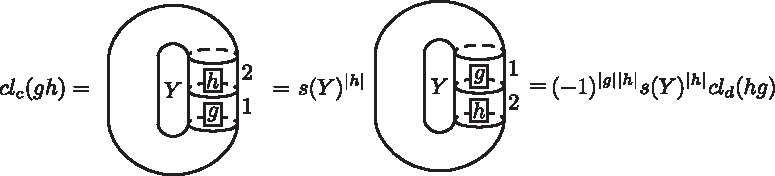
\includegraphics{KernalCl.pdf}
\caption{ A graphical illustration of how to interchange morphisms in the tube category. 
The labels $1$ and $2$ denote the order in which the morphisms $g$ and $h$ appear in 
tensor products. The factor of $s(Y)$ comes from transporting $h$ around the torus, and the factor of 
$(-1)^{|g||h|}$ 
%comes from the super-commutativity of the tensor product. 
is the usual Koszul sign.
}
\label{KernalCl} 
\end{center}
\end{figure}

\item In fact, elements of the form \eqref{cl_ker} generate all of the kernel of $\cl$.
In the bosonic case, this is a standard fact (see \cite{Walker2006}).
The proof for the fermionic case is exactly the same, except that we have to keep track of
Koszul signs and signs coming from the spin structure.
The key idea of the proof is that any isotopy of the torus can be decomposed into (a) isotopies which
are fixed near $K$, and therefore can be lifted to isotopies of the annulus, and (b) a ``shift" isotopy
as described above.
In summary,
\be \label{torus_thm}
	A(T_{XY}) \cong \left( \bigoplus_x \End(x) \right) / \left\langle gh - (-1)^{|g| |h|} s(Y)^{|h|} hg \right\rangle .
\ee

\item In the semisimple case, the expression \eqref{torus_thm} can be greatly simplified.
Let $\{e_i\}$ be a complete set of minimal idempotents for $\tube^X$.
Any endomorphism $f$ can be written as a sum of endomorphisms of the form $f' e_i f''$.
Using \eqref{cl_ker}, we see that the subspace (of the big direct sum)
\be
	\bigoplus_i \End(e_i)
\ee
maps surjectively to $A(T_{XY})$.
Furthermore, because the minimal idempotents are orthogonal (in the sense that $e_i f e_j$ is zero for any $f$ unless $i=j$),
the only relations we have to consider are of the form
\be \label{t2_idem_rels}
	gh - (-1)^{|g| |h|} s(Y)^{|h|} hg
\ee
where both $g$ and $h$ are endomorphisms of $e_i$.
The theorem now follows.
\end{enumerate}

If $e_i$ is m-type, then \eqref{t2_idem_rels} is always zero and we get a summand of $\cc^{1|0}$ in $A(T_{XY})$.
If $e_i$ is q-type and $Y$ is $B$, then any odd endomorphism is of the form $\eqref{t2_idem_rels}$
and we get a summand of $\cc^{1|0}$.
If $e_i$ is q-type and $Y$ is $N$, then any even endomorphism is of the form $\eqref{t2_idem_rels}$
and we get a summand of $\cc^{0|1}$.

A useful corollary of Theorem \ref{torus_basis_theorem} is that all the idempotents of 
$\tube^B$ must be m-type.
Since $T_{BN}$ is spin diffeomorphic to $T_{NB}$, we can compute the Hilbert space for 
these spin surfaces in two different ways, one using
idempotents of $\tube^B$ and the other using idempotents of $\tube^N$.
By the first part of the theorem, the Hilbert space of $T_{NB}$ is purely even.
By the second part of theorem, the dimension of the odd part of the Hilbert space of $T_{BN}$
is given by the number of q-type idempotents of $\tube^B$.
Since the two Hilbert spaces are isomorphic, there can be no q-type idempotents in $\tube^B$.

A similar argument shows that the total number of (equivalence classes of) minimal idempotents of $\tube^B$
must equal that of $\tube^N$.



%%%%%%%%%%%%%%%%%%%
\subsection{Fusion rules} \label{fusion_rules}
%%%%%%%%%%%%%%%%%%%

%\kw{
%I think we are currently using (at least) 
%three different notations for the two different vector spaces we might want to associate
%to a surface: $A$, $V$ and $\mch$.
%We should try to make this more consistent.
%In most of my papers and talks, I use $A$ for string nets mod relations, 
%and $Z$ for the dual space of $A$.
%Strictly speaking, $Z$ is the Hilbert space; $A$ could be called the pre-dual Hilbert space.
%In the finite/semisimple case, $A$ and $Z$ are isomorphic, so one does not need to make a big deal about the distinction.
%In any case, I think we should try to be more consistent with the notation.
%I admit that I am probably responsible for most of the notational inconsistency.}
%\ethan{Agreed. I replaced $V(Y)$ with $A(Y)$ in the following discussion.}

In this subsection, we will define the fusion (tensor product) of representations of the tube category.

We begin with some general observations.
Let $Y$ be a spin surface with $k$ boundary components, denoted by $S_1,\ldots,S_k$.
Let $T_i$ denote the tube category corresponding to the circle $S_i$.
Each $T_i$ is (non-canonically) isomorphic to either $\tube^B$ or $\tube^N$.
(In order to make the isomorphisms canonical, we must choose a spin framing in each
boundary component.)
%\footnote{Here we mean the 
%restriction of the full tube category $\tube \cong \tube^B \oplus \tube^N$ to the sector with 
%spin structure given by the spin structure on $S_i$. 
%That is, $T_i = \tube^B$ ($=\tube^N$) if $S_i$ is bounding (non-bounding).}.
Given objects $c_i$ of $T_i$, for $1\le i \le k$, we have a super vector space $A(Y; c_1,\ldots,c_k)$ consisting on string nets
on $Y$, modulo local relations, with boundary conditions $c_i$ at $S_i$.

We can then glue morphisms of $T_i$ (tubes) onto $S_i$ to obtain a new string net with (possibly) different boundary condition.
A concise way to describe this algebraic structure is to say that the collection of super vector spaces $\{A(Y; c_1,\ldots,c_k)\}$
(for all possible values of $c_1,\ldots,c_k$)
affords a representation of the category $T_1\times\cdots\times T_k$.
We will denote this representation by $A(Y)$.

To define the fusion rules of excitations, we take $Y$ to be the 
pair of pants (a.k.a three-punctured sphere), which we will denote as $P$. 

There are four spin structures on $P$. 
In one of them, all three boundary components have a bounding spin structure, while in 
the remaining three, two out of the three boundary components have a non-bounding spin structure.
We will choose a standard representative for each of these spin pairs of pants, 
so that each boundary component is equipped with a spin diffeomorphism to a 
standard copy of $S^1_B$ or $S^1_N$.

Let $T_a$, $T_b$ and $T_c$ denote the three copies of the tube category associated to the boundary components of $P$.
Given representations $\rho_a$ and $\rho_b$ of $T_a$ and $T_b$, we can define a new representation of $T_c$,
denoted $\rho_a\tp\rho_b$, via
\be  \label{tctpdef}
	\rho_a\tp\rho_b = (\rho_a \boxtimes \rho_b) \tp_{T_a\times T_b} A(P) .
\ee
Here $\rho_a \boxtimes \rho_b$ denotes the ``outer" tensor product (so that $\rho_a \boxtimes \rho_b$ is a representation of $T_a\times T_b$), 
and $A(P)$ is the 
trimodule defined above, built out of
vector spaces of string-net configurations (modulo local relations) on $P$ with all possible boundary conditions. 
Informally, $\rho_a\tp \rho_b$ is found by taking a superposition of tubes carrying $\rho_a$ and $\rho_b$ 
(which is the outer product $\rho_a\boxtimes\rho_b$) and gluing them onto a pair of pants (given by $A(P)$). 
The algebraic implementation of gluing is the tensor product $\tp_{T_a\times T_b}$. 

If $\rho$ is the representation (i.e.\ module) determined by an idempotent $e$ (as described at the start of \ref{C2_fusion_rules}),
then the above association of $\rho$ to a boundary component is equivalent to imposing $e$ as a boundary condition
in a annular neighborhood of that boundary component.

%Note that the spin structure grading of the tube category (and its modules) is respected by the above tensor product: \ethan{added some tubes to make it slightly more explicit}
%\begin{align}
%\tube^B \tp \tube^B \cong \tube^B \quad \quad \tube^B \tp \tube^N \cong \tube^N \quad \quad \tube^N \tp \tube^N \cong \tube^B .
%\end{align}

Note that the spin structure grading of the tube category (and its modules) is respected by the above tensor product:
\begin{align}
B \tp B = B \quad \quad B \tp N = N \quad \quad N \tp N = B
\end{align}
where $B$ $(N)$ is shorthand for the bounding (non-bounding) sector of the tube category.

\begin{comment}
\kw{We define $V^{ab}_c$ elsewhere, so probably no need to to it again here.}

\kw{This paragraph needs work.
Should probably use idempotents instead of representations.
I will do more editing later.}
For fixed representations $\rho_a,\rho_b,\rho_c$ of $T_a,T_b,T_c$ on the three boundary components of $P$,
we will define the fusion space $V^{ab}_{c}$ to be the vector space of string-nets on $P$ modulo local relations.
\kw{Need to mention boundary conditions (idempotents) for $P$.}
$V^{ab}_{c}$ is thus given by the collection of maps from the two boundaries of $P$ with $\rho_a,\rho_b$ 
boundary conditions to the boundary of $P$ with $\rho_c$ boundary conditions, and so we can also write $V^{ab}_{c}$ as
\begin{align}
\label{morpants}
V^{ab}_{c} \cong \text{mor}( \underset{a}{\TubeBCx{Q}} \tp \underset{b}{\TubeBCx{R}}  \rightarrow \underset{\;\; \;\; \quad c \in a\tp b}{\TubeBCx{Q+R}} ), 
\end{align}
where $Q, R \in \{ B,N \}$ denote the spin structures of the two punctures being fused. 
This means that $V^{ab}_c$ is the vector space of string-nets modulo local relations on the following pair of pants:
\be \mathord{\vcenter{\hbox{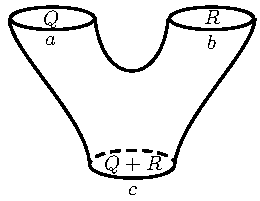
\includegraphics[scale=1]{fusion_space_pants.pdf}}}}.\ee

Finally, we comment on the expression $Q+R$ for the spin structure of $T_c$. 
Since contractible loops are assigned anti-periodic boundary conditions, $B$ acts as $0$ and $N$ 
acts as $1$ when calculating $Q+R$ (where addition is carried out in $\zt$), and 
so the addition rule is 
\begin{align}
B+B = B \quad \quad B+N = N \quad \quad N+N  = B.
\end{align}

\end{comment}


\begin{comment}

 %%%%%%%%%%%%%%%%%%%%%%%%%%%%%%%%%%%%
\subsection{The double braid in terms of the topological twists}
%%%%%%%%%%%%%%%%%%%%%%%%%%%%%%%%%%%%
\dave{Also punt this subsection to future work that includes braiding?}



In this brief section, we comment on an alternate way of calculating the matrix $\mcb^2$ of double braids (mutual statistics). 
Instead of tracing out the $R$ matrices as we did in our analysis of the $C_2$ theory, we can appeal to a formula relating the $\mcb^2$ matrix to the topological twists. 
In bosonic theories, we have the relation
\be 
[{\mcb^2_{bos}}]_{ab} = \frac{1}{\mcd} \sum_c d_c N^{ab}_c \frac{\theta_c}{\theta_a\theta_b}.
\label{stwist_bosonic} 
\ee
This relation does {\it not} hold in the superfusion case, and needs to be modified. 
The derivation of the correct version of \eqref{stwist_bosonic} relies on the fact that
\be \label{stwist_fermionic} \theta_c = (-1)^{|v|(s(c)+1)} \theta_a\theta_b [R^{ab}_c]_{vv} [R^{ba}_c]_{vv},\ee
where $v\in V^{ab}_c$ is any vector in the fusion space $V^{ab}_c$ and $|v| \in \{0,1\}$ is 
the parity of $v$, and where the sum runs over the minimal idempotents of $\tube(\mcc)$.  
Additionally, we have defined the function $s$ by $s(c) = 0$ if $c\in\tube^B(\mcc)$ and $s(c)=1$ if $c\in\tube^N(\mcc)$. 

To derive \eqref{stwist_fermionic}, we use the following manipulations:
\be\label{stwist_proof} 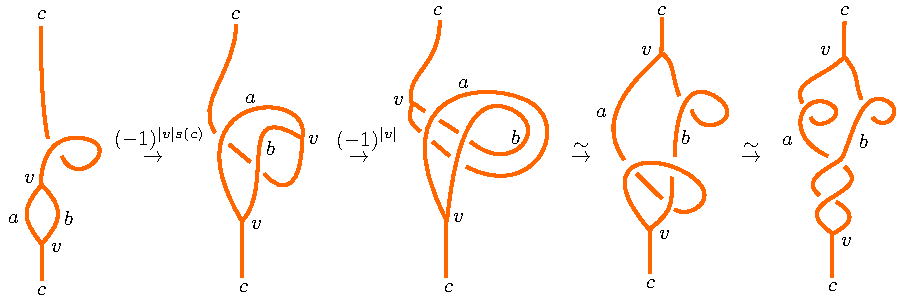
\includegraphics{stwist_proof.pdf}, \ee
where $a$ and $b$ are such that $N^{ab}_c\neq0$, $v$ is any vector in the fusion space $V^{ab}_c$, 
and for clarity we have used the orange lines to represent collections of tubes hosting the quasiparticles $a,b,c$. 
These steps relate something proportional to $\theta_c$ (the leftmost diagram) to something 
proportional to $\theta_a\theta_b [R^{ab}_c]_{vv}[R^{ba}_c]_{vv}$. 
In the bosonic case this relation is an exact equality, but this is not true in the fermionic setting. 
Firstly, we see that the first step in \eqref{stwist_proof} involves passing the vertex $v$ under a $c$ tube. 
When the braiding process is embedded in $S^3$, the branch cuts associated with vortex-type 
quasiparticles become branch sheets, which we will define to always be pointing out of the page. 
This means that passing an odd vector in $V^{ab}_c$ over a vortex-type quasiparticle gives a phase factor of $-1$.
 Additionally, we notice that vectors in $V^{ab}_c$ are transported in a loop during steps 1 and 2, 
 which contributes a sign of $-1$ if the vector $v$ is odd. 
 These two effects are responsible for the factor of $(-1)^{|v|(s(c)+1)}$ in \eqref{stwist_fermionic}, 
 meaning that the correct expression for $\mcb^2$ in the fermionic setting is 
\be [\mcb^2]_{ab} = \frac{1}{\mcd} \sum_c \sum_{v \in V^{ab}_c} d_c (-1)^{|v| (s(c)+1)}   \frac{\theta_c}{\theta_a\theta_b}.\ee 

\end{comment}


%%%%%%%%%%%%%%%%%%%%%%%%%%%%%
\subsection{Dimension formula}
%%%%%%%%%%%%%%%%%%%%%%%%%%%%%

In this subsection we give a Verlinde-type formula for the super dimension of the Hilbert space of a surface $Y$.


\subsubsection{The formula}   \label{dimformula_ss}

Let $Y$ be a spin surface with boundary components $U_1, \ldots, U_k$.
Each $U_i$ inherits either a bounding (a.k.a.\ antiperiodic or non-vortex) spin structure or a nonbounding 
(a.k.a.\ periodic or vortex) spin structure.

Let $a_1,\ldots, a_k$ be a set of labels for $\bd Y$.
Each $a_i$ is a minimal idempotent in the tube category $\tube^{U_i}(\mcc)$
(which is isomorphic to either $\tube^B(\mcc)$ or $\tube^N(\mcc)$); 
either a non-vortex anyon or a vortex anyon
(according to the spin structure on $U_i$).
%%KW I changed notation
%\dave{Maybe we should say $\tube^B(\mcc)$ or $\tube^N(\mcc)$ just to be clear.
%It may be confusing for the reader since we usually put categories into $\tube$ and not $S^1$'s. 
%}
The predual Hilbert space of string-net configurations on $Y$ with boundary conditions 
determined by the $a_i$ is $A(Y; a_1,\ldots, a_k) \cong \cc^{p|q}$ for some integers $p,q$.
Our goal is to compute $p$ and $q$.

\medskip

Let $S_{ab}$ denote the normalized, unitary $S$-matrix.
The indices $a$ and $b$ are closed-up idempotents on a spin torus.
They are specified by giving an idempotent (either bounding or nonbounding) together with
the way the annulus was glued 
%%KW: "longitudinal" is confusing because the S matrix involves cutting along two orthogonal cycles
%along the longitudinal direction 
to obtain the torus (again either bounding or nonbounding,
independent of the bounding/nonbounding status of the idempotent).
The idempotent $a$ is glued up in a (non)bounding way if $b$ is a (non)bounding idempotent, 
and vice versa.\footnote{
%%KW I don't we need to mention embeddings on $S^3$; diffeomorphisms of T^2 should suffice
%\ethan{In brief, this constraint can be seen from writing $S_{ab}$ as the partition function of two 
%linked tori embedded in $S^3$, with the tori corresponding to the closed-up idempotents $a$ and $b$.
%Requiring that the linked tori embed into $S^3$ (so that there are no free spin structure defect 
%endpoints) enforces that the spin structure along the longitudinal cycle of one torus match the spin 
%structure along the meridional cycle of the other.}
This is because spin structure on the cutting circle of one torus must
match the spin structure of the circle perpendicular to the cutting circle of the other torus.
%%KW not completely happy with above
}
%%KW: broken reference; deleting for now
%(see the discussion around Figure \ref{braided_tubes}).
If the idempotent is q-type, it is rescaled by $1/\sqrt 2$ to obtain a unit vector in $A(T^2)$, 
the vector space of string-net configurations modulo local relations on the torus
(see \ref{traces_and_innerproducts}).
(Note that there is still some ambiguity for entries in the $S$-matrix corresponding
to odd vectors in $T^2_{NN}$, but the formulas below will not use these $S$-matrix entries.)

Let $S'_{ab}$ be $S_{ab}$ if $a$ is m-type and $\sqrt 2 \cdot S_{ab}$ if $a$ is q-type.
Note that $S'_{ab}$ is asymmetric in $a$ and $b$;
we're undoing the normalization for $a$ but not for $b$.
The idempotents we will be summing over fall into three classes:
$B_m$ (bounding and m-type), $N_m$ (non-bounding and m-type), and $N_q$ (non-bounding and q-type).
Recall 
%(from the discussion after \eqref{tube_spin_decomp}) 
(from the discussion at the end of \ref{ground_states_on_torus}) 
that bounding idempotents are always m-type; in other words the potential fourth class $B_q$ is empty.


\medskip

We can now state the dimension formula:
We have
\be
	p + q = \sum_{x\in B_m} {S_{1x}}^{\chi(Y)} {\textstyle \prod_i} S'_{a_i x} 
	\label{PplusQ}
\ee
where $\chi(Y)$ is the Euler characteristic of $Y$.
If any of the $a_i$ are q-type, then we know that $p=q$ and we are done, since in that case 
$\cc^{p|q}$ has an odd isomorphism coming from the action of an odd element of $\End(a_i)$.

Now assume that none of the $a_i$ are q-type.
In this case we have
\be
	p - q = \sum_{x\in N_m} {S_{1x}}^{\chi(Y)} {\textstyle \prod_i} S'_{a_i x}
			\;\;+\;\; (-1)^{\Arf(Y)} \sum_{x\in N_q} {S_{1x}}^{\chi(Y)} {\textstyle \prod_i} S'_{a_i x} .
			\label{PminusQ}
\ee
Where $\Arf(Y)$ is the Arf invariant of $Y$.
If $Y$ is closed, then $\Arf(Y) = 0$ if $Y$ has a bounding spin structure and 
$\Arf(Y) = 1$ if $Y$ has a nonbounding spin structure.
For a torus, the $BB$, $BN$ and $NB$ spin structures are bounding and the $NN$ spin structure is nonbounding.
$\Arf(Y)$ for a higher genus spin surface can be determined by writing $Y$ as a connected sum of spin tori,
and using the fact that $\Arf(Y)$ is additive under connected sums.

If $Y$ has non-empty boundary and each boundary component has a bounding spin structure, 
we define $\Arf(Y)$ to be the Arf invariant of the closed 
surface obtained by capping each boundary component off with a disk.

If $Y$ has a non-bounding boundary component, say $U_1$, then by assumption
the label $a_1$ is m-type.
It follows that $S'_{a_1 x} = 0$ if $x$ is q-type, so there is no need to define $\Arf(Y)$ in this case.
We can see that $S'_{a_1 x} = 0$
because the torus basis vector corresponding to $x$ is odd (odd endomorphism of $x$
glued up periodically), while the basis vector corresponding to $a_1$ is even (the idempotent $a_1$
glued up periodically), and $S$ is an even operator.
This can be observed, for example, the $NN$ block of the $S$-matrix
for the $\halfesix/\psi$ theory, \eqref{hE6_S_NN}.

Note that the formula for $p+q$ above does not depend on the Arf invariant of $Y$, while the formula for $p-q$ does.
Thus the total dimension of the Hilbert space is not sensitive to the spin structure
of $Y$, but the even and odd Hilbert space dimensions do depend on the spin structure.



\subsubsection{Sketch of proof}

In this subsection we sketch the proof of the above dimension formula.

\newcommand{\ztt}{Z}
\newcommand{\zob}{Z_{S^1_B}}
\newcommand{\zon}{Z_{S^1_N}}


Let $\ztt$ denote the $2{+}1$-dimensional TQFT associated to the super pivotal category $\mcc$.
Let $Y$ be a closed spin surface with Hilbert space $\ztt(Y)$, and let $p|q = \dim(\ztt(Y))$.
Then we have
\be  \label{df1}
	p+q = \tr(\id: \ztt(Y) \to \ztt(Y)) = \ztt(Y\times S^1_B)
\ee
and
\be  \label{df2}
	p-q = \tr((-1)^F: \ztt(Y) \to \ztt(Y)) = \ztt(Y\times S^1_N) .
\ee
%yay! confirms our earlier suspicions about supertraces 
More generally, if $Y$ has nonempty boundary and the boundary components are labeled by $a_1,\ldots,a_k$ 
(minimal idempotents of the tube category), then
\begin{align}  \label{df3}
	p+q & = \tr(\id: \ztt(Y; a_1,\ldots,a_k) \to \ztt(Y; a_1,\ldots,a_k)) \\
		& = \ztt(Y\times S^1_B)(\cl_B(a_1)\du\cdots\du \cl_B(a_k))
\end{align}
and
\begin{align}  \label{df4}
	p-q & = \tr((-1)^F:  \ztt(Y; a_1,\ldots,a_k) \to \ztt(Y; a_1,\ldots,a_k)) \\
		& = \ztt(Y\times S^1_N)(\cl_N(a_1)\du\cdots\du \cl_N(a_k)) .
\end{align}
Here $\cl_X(a_i)$ denotes the element of $\ztt(T^2_{UX})$ obtained by closing up the idempotent $a_i$,
and $U$ is the spin structure ($B$ or $N$) on the $i$-th boundary component.
Note that if $a_i$ is q-type, then $\cl_N(a_i) \in \ztt(T^2_{NN})$ is zero.
But in this case we also know that $p-q = 0$, since the odd endomorphism of $a_i$ maps the even part of 
$\ztt(Y; a_1,\ldots,a_k)$ isomorphically to the odd part.

\medskip

Recall that we can define reduced $1{+}1$-dimensional TQFTs $\zob$ and $\zon$ via
\be
	\zob(M) = \ztt(M\times S^1_B) \quad\quad \zon(M) = \ztt(M\times S^1_N) ,
\ee
where $M$ is a manifold of dimension 0, 1 or 2.
Combining the above we have, for closed spin surfaces $Y$,
\be  \label{df5}
	p+q = \zob(Y)
\ee
and
\be  \label{df6}
	p-q = \zon(Y) ,
\ee
and there are similar formulas when $Y$ has boundary.

\medskip

We can now outline the remainder of the proof of the dimension formula.
We have just seen that the super dimension $p|q$ can be calculated entirely in terms of the reduced 
$1{+}1$-dimensional TQFTs $\zob$ and $\zon$.
Because 1 is a small number, we can completely classify $1{+}1$-dimensional spin TQFTs and give an explicit
expression for the path integral in terms of basic structure constants of the $1{+}1$-dimensional TQFT.
Then all that remains to be done is express the structure constants of the $1{+}1$-dimensional TQFTs in terms
of the structure constants of the original $2{+}1$-dimensional TQFT $\ztt$.
It turns out that the only structure constants we will need are the list of minimal idempotents of the tube category, 
their types (m or q), and the $S$-matrix.

\medskip

Spin $1{+}1$-dimensional TQFTs are determined by two pieces of data:
the cylinder category of a point, which is a linear super category $C$,
and a non-degenerate trace on $C$.
The trace is the path integral of the disk $D^2$; if $f$ is an endomorphism of $C$, then
\be
	\tr(f) = Z_{C,\tr}(D^2)(\cl(f)) ,
\ee
where, as usual, $\cl(f)$ denotes the closure of $f$, an element of the (pre-dual) Hilbert space associated to $S^1_B = \bd D^2$.
The non-degenerate trace implies that $C$ is semisimple.
Up to Morita equivalence, there are only two indecomposable semisimple super categories, the 
trivial algebra $\cc$ and the complex Clifford algebra $\cliff_1$.

We first consider the case $C = \cc$.
Let $e$ be the unique minimal idempotent of $\cc$ (i.e.\ $e = 1\in \cc$).
Let $\lambda = \tr(e)$.
Let $Y$ be a spin surface with $k$ boundary components, and let
$\cl(e)\du\cdots\du \cl(e)$ denote the boundary condition given by placing $\cl(e)$ on each boundary component of $Y$.
The the path integral for the TQFT determined by $(\cc, \lambda)$ is
\be  \label{zc_ans}
	Z_{\cc,\lambda}(Y)(\cl(e)\du\cdots\du \cl(e)) = \lambda^{\chi(Y)} ,
\ee
where $\chi(Y)$ denotes the Euler characteristic of $Y$.

Next we consider the case $C = \cliff_1$.
Again let $e$ be the unique minimal idempotent of $\cliff_1$.
Let $\lambda = \tr(e)$.
Let $Y$ be a spin surface with $k$ boundary components.
We will assume that each boundary component of $Y$ has the bounding spin structure, since that is the only case
we will need for the dimension formula.
Let
\be
	\hat e = \frac{1}{\sqrt 2} \, e
\ee
be the normalized idempotent.
(The norm of $\cl(\hat e)$ in $A(S^1_B)$ is 1.)
The the path integral for the TQFT determined by $(\cliff_1, \lambda)$ is
\be \label{zcl1_ans}
	Z_{\cliff_1,\lambda}(Y)(\cl(\hat e)\du\cdots\du \cl(\hat e)) = (-1)^{\Arf(Y)} \left(\frac{\lambda}{\sqrt 2}\right)^{\chi(Y)} ,
\ee
where $\chi(Y)$ denotes the Euler characteristic of $Y$,
and $\Arf(Y)$ is the Arf invariant of $Y$ with its boundary components capped off by disks.

A general $1{+}1$-dimensional spin TQFT is a direct sum of instances of the two theories described above.

\medskip

All that remains to be done is to write the reduced theories $\zob$ and $\zon$ as a direct sum of the $(\cc, \lambda)$ and
$(\cliff_1, \lambda)$ theories described above.

The first task is to obtain a list of the idempotents (and their type, m or q) of the minimal
idempotents of $\zob$ and $\zon$.
This is easily done: the category which $\zob$ assigns to a point is $\tube^B$, and the 
category which $\zon$ assigns to a point is $\tube^N$.
The m-type idempotents correspond to $(\cc,\lambda)$ theories, and the q-type idempotents
correspond to $(\cliff_1,\lambda)$ theories.

The second task is to determine, for each idempotent $a$ in $\tube^B$ and $\tube^N$,
the number $\lambda$ above (path integral of the disk evaluated on a closed-up idempotent).
This is exactly the $S$-matrix entry $S_{1a}$ if $a$ is m-type.
If $a$ is q-type, then (since we have normalized the $S$-matrix) $S_{1a}$ is equal to $\lambda/\sqrt 2$, but this
is the value we need for \eqref{zcl1_ans}.

The third and final task is to convert the $\cl(a_i)$ boundary conditions from the beginning of \ref{dimformula_ss}
to the $\cl(e)$ and $\cl(\hat e)$ boundary conditions appearing in \eqref{zc_ans} and \eqref{zcl1_ans}.
Both of these boundary conditions are (after undoing the dimensional reduction along $S^1_B$ or $S^1_N$) vectors
in $A(T^2)$, and both boundary conditions are closed-up idempotents (possibly normalized with a factor of $1/\sqrt 2$).
But the $\cl(a_i)$ boundary condition cuts the torus along a longitude, while the $\cl(e)$ and $\cl(\hat e)$ boundary conditions
cut the torus along a meridian.
So we need to apply the $S$-matrix (actually $S'$, because $\hat e$ is normalized while $a_i$ is not) to change basis:
\be  \label{df_cob}
	\cl(a_i) = \sum_x S'_{a_ix} \cl(\hat x),
\ee
where for convenience we have defined $\hat x = x$ if $x$ is m-type.

Combining \eqref{df5}, \eqref{df6}, \eqref{zc_ans}, \eqref{zcl1_ans}, and \eqref{df_cob}
yields the dimension formula.





\subsubsection{Sample calculations}

\begin{figure}\begin{center}  \tabulinesep = 1mm
\begin{tabu}{|X[$l]|X[$c]|X[$c]|X[$c]|}
	\hline
	& C_2 & SO(3)_6/\psi & \halfesix/y \\ \hline
	g=1, \Arf = 0 & 3 \;|\; 0 & 4 \;|\; 0 & 3 \;|\; 0  \\ 
	g=1, \Arf = 1 & 0 \;|\; 3 & 2 \;|\; 2 & 1 \;|\; 2  \\ \hline
	g=2, \Arf = 0 & 10 \;|\; 0 & 40 \;|\; 24 & 19 \;|\; 8  \\
	g=2, \Arf = 1 & 0 \;|\; 10 & 32 \;|\; 32 & 11 \;|\; 16  \\ \hline
	g=3, \Arf = 0 & 36 \;|\; 0 & 1184 \;|\; 1120 & 281 \;|\; 232  \\
	g=3, \Arf = 1 & 0 \;|\; 36 & 1152 \;|\; 1152 & 241 \;|\; 272  \\ \hline
	g=4, \Arf = 0 & 136 \;|\; 0 & 51328 \;|\; 51072 & 5755 \;|\; 5504  \\
	g=4, \Arf = 1 & 0 \;|\; 136 & 51200 \;|\; 51200 & 5531 \;|\; 5728  \\ \hline
	g=5, \Arf = 0 & 528 \;|\; 0 & 2368000 \;|\; 2366976 & 126449 \;|\; 125056  \\ 
	g=5, \Arf = 1 & 0 \;|\; 528 & 2367488 \;|\; 2367488 & 125137 \;|\; 126368  \\ \hline
\end{tabu}
\caption{Hilbert space dimensions for closed surfaces in various theories.} \label{dim_formula_fig1}
\end{center}\end{figure}


There are three specific $S$ matrices calculated in this paper, for the TQFTs based on the $C_2$, $SO(3)_6/\psi$, and $\halfesix/y$ theories.
%%KW change made, though I don't see why one version is less confusing than the other
%\dave{I didn't want the reader to think we wrote down S-matrices for e.g., $C_2$, but for the TQFT %turaev viro theory made out of $C_2$. }
%\dave{To avoid confusion we could say:
% `There are three specific $S$ matrices calculated in this paper, for the TQFTs based on the $C_2$, $SO(3)_6/\psi$, and $\halfesix/\psi$ theories.'}
Note that all three of these theories have just one non-trivial simple object.
Plugging the $S$-matrix entries into the above dimension formula, we find, for closed surfaces of genus $g$ and specified Arf invariant,
the results in Figure \ref{dim_formula_fig1}.
%\kw{Maybe better to make eqn rather than figure??}

\kw{added:}
\kw{Will add daves suggestion}
\dave{That's a useful remark, and one of the most useful instances of this formula. 
Maybe we should just write out the formula explicitly (with factors of $\sqrt{n_{a_i}}$) in this case.
It looks very similar to the familiar formula $N_{ab}^c = \sum_x SSS/S$, which some people may enjoy.
I can do this if we think it's a good idea.}
If we take $Y$ to be a 3-punctured sphere (with various spin structures),
then we can use the dimension formula to compute the fusion rules of the tube category.
For example, the fusion rules of Table \ref{TubehalfesixFusionRules} were computed using
the dimension formula.

We remark that the dimension formula is a useful check on $S$-matrix accuracy.
Mistakes in calculating the $S$ matrix typically lead to non-integer outputs from the dimension formula.
%\kw{Remark that this is a good way to detect errors in S? (most errors lead to non-integer dims)}


%\kw{Should also do some examples for surfaces with boundary.
%e.g.\ odd fusion channels in C2, odd self-duality in E6/2/p, genus two surface with two labeled boundary components}

%\kw{Is it worthwhile to write out the sums for some of the calculations?}
